\documentclass{amsart}
\usepackage{amsmath}
\usepackage{amssymb}
\usepackage{latexsym}
\usepackage{color}
%\usepackage{ulem}
\usepackage[margin=1in]{geometry}
\usepackage{tikz}
\usetikzlibrary{math}
\usepackage[bookmarks=true, bookmarksopen=true, bookmarksdepth=3,bookmarksopenlevel=2, colorlinks=true, linkcolor=blue, citecolor=blue, filecolor=blue, menucolor=blue, urlcolor=blue]{hyperref}

\usepackage[draft]{say}
\newcommand{\sayDR}[1]{\say[DR]{\color{red}{\bf DR:}\;#1}}
\newcommand{\saySS}[1]{\say[SS]{\color{blue}{\bf SS:}\;#1}}

\newtheorem{theorem}{Theorem}
\newtheorem{corollary}[theorem]{Corollary}
\newtheorem{definition}[theorem]{Definition}
\newtheorem{lemma}[theorem]{Lemma}
\newtheorem{proposition}[theorem]{Proposition}
\newtheorem{remark}[theorem]{Remark}
\newtheorem{conjecture}[theorem]{Conjecture}
\newtheorem{question}{Question}

\numberwithin{theorem}{section}

\newcommand{\bfa}{\boldsymbol{a}}
\newcommand{\bfc}{\boldsymbol{c}}
\newcommand{\bfg}{\boldsymbol{g}}
\newcommand{\bfr}{\boldsymbol{r}}
\newcommand{\bfx}{\boldsymbol{x}}
\newcommand{\bfy}{\boldsymbol{y}}

\newcommand{\cA}{\mathcal{A}}
\newcommand{\cC}{\mathcal{C}}
\newcommand{\cD}{\mathcal{D}}
\newcommand{\cI}{\mathcal{I}}
\newcommand{\cP}{\mathcal{P}}
\newcommand{\cQ}{\mathcal{Q}}
\newcommand{\cS}{\mathcal{S}}

\newcommand{\fp}{\mathfrak{p}}

\newcommand{\CC}{\mathbb{C}}
\newcommand{\QQ}{\mathbb{Q}}
\newcommand{\RR}{\mathbb{R}}
\newcommand{\TT}{\mathbb{T}}
\newcommand{\ZZ}{\mathbb{Z}}

\newcommand{\ol}[1]{{\overline{#1}}}
\newcommand{\vv}[1]{{{}^\vee \! #1}}

\newcommand{\Aut}{\operatorname{Aut}}
\newcommand{\Col}{\operatorname{Col}}
\newcommand{\diag}{\operatorname{diag}}
\newcommand{\dpt}{\operatorname{dp}}
\newcommand{\hgt}{\operatorname{ht}}
\newcommand{\Id}{\operatorname{Id}}
\newcommand{\into}{\hookrightarrow}
\newcommand{\obeta}{{\overline{\beta}}}
\newcommand{\oi}{{\overline{\imath}}}
\newcommand{\ot}{{\overline{t}}}
\newcommand{\rsh}{{\operatorname{rsh}}}
\newcommand{\sh}{{\operatorname{sh}}}
\newcommand{\WA}{{W\!\!A}}
\newcommand{\wt}{{\operatorname{wt}}}

\newcommand{\kk}{\Bbbk}

\title{Dominance Regions for Rank Two Cluster Algebras}

\author{Dylan Rupel}
\author{Salvatore Stella}

\begin{document}
  \begin{abstract}
    We investigate the shapes of the polytopes defining the dominance order for $\bfg$-vectors in cluster algebras of rank two.
    We arrive at a complete description: 
    \begin{itemize}
      \item cluster monomials are never deformable;
      \item the imaginary dominance polytopes are kites, triangles, or trapezoids which extend far outside the imaginary cone; the triangles appearing along rays corresponding to columns of the associated Cartan matrix.
    \end{itemize}
  \end{abstract}
  \maketitle

  \section{Introduction}
  Cluster algebras were introduced by Fomin and Zelevinsky as a tool in the study of Lusztig's (dual) canonical bases.
  Since their inception they have found application in a variety of different areas in mathematics, nevertheless a fundamental problem in the theory remains constructing bases with ``good'' properties. 
  
  Over time several bases for cluster algebras have been constructed in a variety of generalities \cite{foo,bar,baz}. 
  All of them share a property of being ``pointed''.
  Being pointed turned out to be a desirable feature for a basis to have and a natural question is to find all bases enjoying this property.
  Recently Qin introduced the notion of \emph{dominance} and showed that it completely encapsulates the deformability of pointed bases whenever the cluster algebra has full rank \cite{Qin}. 
  As no explicit calculation is carried out in his work, we aim here at describing explicitly the space of deformability for pointed bases in rank two, i.e. when clusters contain a pair of mutable cluster variables.
  In this setting, frozen variables do not carry any additional information and we can work in the coefficient-free case. 

  Fix integers $b,c>0$.  The cluster algebra $\cA(b,c)$ is the $\ZZ$-subalgebra of $\QQ(x_0,x_1)$ generated by \emph{cluster variables} $x_m$, $m\in\ZZ$, defined recursively by
  \begin{equation}
    x_{m-1}x_{m+1}=\begin{cases} x_m^b+1 & \text{if $m$ is even;}\\ x_m^c+1 & \text{if $m$ is odd.} \end{cases}
  \end{equation}
  By the Laurent Phenomenon \cite{fomin-zelevinsky}, each $x_m$ is actually an element of $\ZZ[x_k^{\pm1},x_{k+1}^{\pm1}]$ for any $k\in\ZZ$.
  Moreover, these Laurent polynomials are known to have positive coefficients \cite{LLZ,lee-schiffler,GHKK}.

  Our goal in this note is to explicitly compute the possible bases which are pointed with respect to the embedding $\cA(b,c)\into\ZZ[x_k^{\pm1},x_{k+1}^{\pm1}]$ for every $k\in\ZZ$.
  That is, a basis element with \emph{$\bfg$-vector} $\lambda\in\ZZ^2$ when expanded in terms of $\{x_0,x_1\}$ can be written in the form
  \begin{equation}
    \label{eq:pointed}
    x_0^{\lambda_1}x_1^{\lambda_2}\sum\limits_{a_1,a_2 \ge 0} c^\lambda_{a_1,a_2} x_0^{-ba_1} x_1^{ca_2}
  \end{equation}
  with $c^\lambda_{0,0}=1$.
  Being \emph{pointed} means an analogous structure reproduces after expanding in terms of any pair $\{x_k,x_{k+1}\}$.
  %The collection of all $\bfg$-vectors $\lambda\in\ZZ^2$ parametrize the elements of any pointed basis.

  Important examples of pointed elements are the \emph{cluster monomials} of $\cA(b,c)$, i.e. the elements that can be written in the form $x_k^{a_1}x_{k+1}^{a_2}$ for some $k\in\ZZ$ and $a_1,a_2$ non-negative integers.
  Indeed, by [someresult of Qin] cluster monomials are part of any pointed basis in any cluster algebra.
  \say{Check if this needs full rank}

  Elements of any pointed basis are parametrized by their $\bfg$-vectors.
  Qin introduced a partial order on $\bfg$-vectors called the \emph{dominance order} and showed that given two pointed bases $x=\{x_\lambda\}$, $y=\{y_\lambda\}$, $y_\mu$ can appear in the expansion of $x_\lambda$ in terms of $y$ only if $\lambda$ dominates $\mu$ (cf. \cite[Mainthm]{Qin} and \ref{below}).

  When $bc\le3$, the cluster algebra $\cA(b,c)$ will be of finite-type and cluster monomials form its only pointed basis.
  We will therefore assume that $bc\ge4$.
  In this case we give an explicit description of the dominance relation among $\bfg$-vectors.
  Specifically, we show that the $\bfg$-vector $\lambda$ dominates the collection of $\bfg$-vectors of the form $\lambda+(b a_1 ,c a_2)$, $a_1,a_2\in\ZZ$, inside its \emph{dominance polygon} $\cP(\lambda)$.
  %In this case, we compute the possible transitions between any two pointed bases.
  %The collection of $\bfg$-vectors which can appear in the deformation of a pointed basis is the \emph{dominance region}.
  \begin{theorem}
    \label{th:dominance inequalities}
    The dominance polygon $\cP(\lambda)$ pointed at $\lambda=(\lambda_1,\lambda_2)$ is the region defined by $x\leq \lambda_1, y\geq\lambda_2$, and the following inequalities:
    {
      \everymath={\displaystyle}
      \def\arraystretch{2.8}
      \[
        \begin{array}{rcccl}
          0 & \leq & \frac{b c-\sqrt{b c (b c-4)}}{2 b}(x-\lambda_1)+(y-\lambda_2) & \leq & \max\left(-c\lambda_1-\frac{b c+\sqrt{b c (b c-4)}}{2b}b\lambda_2,0\right)
          \\
          \min\left(-c\lambda_1,0\right) & \leq & \frac{b c-\sqrt{b c (b c-4)}}{2 b}(x-\lambda_1)-(y-\lambda_2) & \leq & 0
          \\
          0 & \leq &  -(x-\lambda_1)-\frac{b c-\sqrt{b c (b c-4)}}{2 c}(y-\lambda_2) & \leq & \max\left(\frac{b c+\sqrt{b c (b c-4)}}{2c}c\lambda_1+b\lambda_2,0\right)
          \\
          \min\left(b \lambda_2,0\right) & \leq & (x-\lambda_1) - \frac{b c-\sqrt{b c (b c-4)}}{2 c} (y-\lambda_2) & \leq & 0
        \end{array}
      \]
    }
  \end{theorem}

  A number of bases for rank two cluster algebras with various defining properties have been constructed.
  A natural starting basis is the so-called \emph{greedy basis} in which all $c^\lambda_{a_1,a_2}$ are non-negative and these coefficients are chosen to be minimal.
  It is known that this choice coincides with the theta basis \cite{GHKK, CGMMRSW}.
  The \emph{standard monomial bases} of $\cA(b,c)$ come from natural identifications with the subalgebras of $\ZZ[x_0^{\pm1},x_1^{\pm1}]$ generated by $x_{k-1}$, $x_k$, $x_{k+1}$, and $x_{k+2}$ for $k\in\ZZ$.
  However, these bases depend on $k$ and the triangular basis is defined by a triangular transition with the stipulation that the basis does not depend on the choice of starting cluster.
  It would be useful to explicitly (or combinatorially) compute the transitions between these bases.
  However, explicit calculations reveal that the $\bfg$-vectors actually appearing in these transitions are far smaller than the entire dominance polygon.


  \begin{theorem}
    \label{th:dominance vertices}
    There are six classes of dominance polytopes.
    \begin{enumerate}
      \item If $\lambda$ lies outside of $\cI$, i.e. if it is the $\bfg$-vector of a cluster monomial, then $\cP(\lambda)$ is the point $\lambda$. 
      \item If $\lambda$ lies in the interior of the cone spanned by the vectors $(2b,-bc-\sqrt{bc(bc-4)})$ and $(2,-c)$, then $\cP(\lambda)$ is the trapezoid with corner vertices $\lambda$, $-\frac{bc+\sqrt{bc(bc-4)}}{2c}\big(\frac{bc+\sqrt{bc(bc-4)}}{2b}\lambda_1+\lambda_2,0\big)$, $\big(0,\frac{bc+\sqrt{bc(bc-4)}}{2b}\lambda_1+\lambda_2\big)$, and $\frac{bc+\sqrt{bc(bc-4)}}{2\sqrt{bc(bc-4)}}\big(-(bc-2)\lambda_1-b\lambda_2,c\lambda_1+2\lambda_2\big)$.
      \item If $\lambda$ lies on the ray spanned by $(2,-c)$, say $\lambda=(2\ell,-c\ell)$, then $\cP(\lambda)$ is the triangle with corner vertices $\lambda$, $\big(2\ell-\frac{bc+\sqrt{bc(bc-4)}}{2}\ell,0\big)$, and $\big(0,\frac{\sqrt{bc(bc-4)}}{b}\ell\big)$.
      \item If $\lambda$ lies in the interior of the cone spanned by the vectors $(2,-c)$ and $(b,-2)$, then $\cP(\lambda)$ is the kite with corner vertices $\lambda$, $\big(\lambda_1+\frac{bc+\sqrt{bc(bc-4)}}{2c}\lambda_2,0\big)$, $\frac{bc+\sqrt{bc(bc-4)}}{2\sqrt{bc(bc-4)}}(2\lambda_1+b\lambda_2,c\lambda_1+2\lambda_2)$, and $\big(0,\frac{bc+\sqrt{bc(bc-4)}}{2b}\lambda_1+\lambda_2\big)$.
      \item If $\lambda$ lies on the ray spanned by $(b,-2)$, say $\lambda=(b\ell,-2\ell)$, then $\cP(\lambda)$ is the triangle with corner vertices $\lambda$, $\big(-\frac{\sqrt{bc(bc-4)}}{c}\ell,0\big)$, and $\big(0,\frac{bc+\sqrt{bc(bc-4)}}{2}\ell-2\ell\big)$.
      \item If $\lambda$ lies in the interior of the cone spanned by the vectors $(b,-2)$ and $(2b,-bc+\sqrt{bc(bc-4)})$, then $\cP(\lambda)$ is the trapezoid with corner vertices $\lambda$, $\big(\lambda_1+\frac{bc+\sqrt{bc(bc-4)}}{2c}\lambda_2,0\big)$, $-\frac{bc+\sqrt{bc(bc-4)}}{2b}\big(0,\lambda_1+\frac{bc+\sqrt{bc(bc-4)}}{2c}\lambda_2\big)$, and $\frac{bc+\sqrt{bc(bc-4)}}{2\sqrt{bc(bc-4)}}\big(2\lambda_1+b\lambda_2,-c\lambda_1-(bc-2)\lambda_2\big)$.
    \end{enumerate}
  \end{theorem}

  \begin{remark}
    Note that the rays which separate the regions inside $\cI$ correspond exactly to the columns of the associated Cartan matrix $\left[ \begin{array}{cc} 2 & -b \\ -c & 2 \end{array} \right]$.
    This unexpected coincidence is one of our reasons for deciding to write down these results.
  \end{remark}

  Given a Laurent polynomial in $\ZZ[x_0^{\pm1},x_1^{\pm1}]$, its \emph{support} is the set of its exponent vectors inside $\ZZ^2$.
  \begin{theorem}
    \label{th:maximum support}
    For a $\bfg$-vector $\lambda=(\lambda_1,\lambda_2)\in\ZZ^2$ the support for a pointed basis vector $x_\lambda$ is contained in the (possibly degenerate) lattice quadrilateral $\cS_\lambda$ given as follows:
    \begin{enumerate}
      \item If $\lambda$ lies outside of $\cI$, there are the following possibilities:
        \begin{enumerate}
          \item If $0\le\lambda_1,\lambda_2$, then $\cS_\lambda$ is just the point $\lambda$.
          \item If $\lambda_2 < 0$ and $0\le\lambda_1+b\lambda_2$, then $\cS_\lambda$ is the segment joining $\lambda$ and $(\lambda_1+b\lambda_2,\lambda_2)$.
          \item If $\lambda_1 < 0$ and $0\le\lambda_2$, then $\cS_\lambda$ is the segment joining $\lambda$ and $(\lambda_1,-c\lambda_1+\lambda_2)$.
          \item If $\lambda_1,\lambda_2 < 0$, then $\cS_\lambda$ has corner vertices $\lambda$, $(\lambda_1+b\lambda_2,\lambda_2)$, $\big(\lambda_1+b\lambda_2,-c\lambda_1-(bc-1)\lambda_2\big)$, and $(\lambda_1,-c\lambda_1+\lambda_2)$.
          \item If $\lambda_1 > 0$, $\lambda_1+b\lambda_2 < 0$, and $-c\lambda_1-(bc-1)\lambda_2\le 0$, then $\cS_\lambda$ has corner vertices $\lambda$, $(\lambda_1+b\lambda_2,\lambda_2)$, $\big(\lambda_1+b\lambda_2,-c\lambda_1-(bc-1)\lambda_2\big)$, and $\big((bc+1)\lambda_1-b^2c\lambda_2,-c\lambda_1-(bc-1)\lambda_2\big)$.
          \item If $\lambda_1 > 0$, $\lambda_1+b\lambda_2 < 0$, and $0 < -c\lambda_1-(bc-1)\lambda_2$, then $\cS_\lambda$ has corner vertices $\lambda$, $(\lambda_1+b\lambda_2,\lambda_2)$, $\big(\lambda_1+b\lambda_2,-c\lambda_1-(bc-1)\lambda_2\big)$, and $(0,0)$.
        \end{enumerate}
      \item If $\lambda$ lies inside of $\cI$, then $\cS_\lambda$ has corner vertices $\lambda$, $(\lambda_1+b\lambda_2,\lambda_2)$, $\big(\lambda_1+b\lambda_2,-c\lambda_1-(bc-1)\lambda_2\big)$, and $\frac{bc+\sqrt{bc(bc-4)}}{2\sqrt{bc(bc-4)}}\big(2\lambda_1+b\lambda_2,-c\lambda_1-(bc-2)\lambda_2\big)$.
    \end{enumerate}
  \end{theorem}

\begin{figure}[h!]
  \centering
    \newcommand{\setconstants}{
      \tikzmath{\b = 3.5; \c = 4.4 / \b; \s = sqrt(\b * \c * (\b * \c -4)); \bcmo = \b * \c - 1; \bcms = \b * \c - \s; \bcps = \b * \c + \s;}
      \tikzmath{ \xmin = -6; \xmax = 6; \ymin = -6; \ymax = 6;}
      \clip (\xmin,\ymin) rectangle (\xmax,\ymax);
    }
    \newcommand{\boundingrays}{
      \draw [color=lightgray, thick] (2*\xmin,0) -- (2*\xmax,0);
      \draw [color=lightgray, thick] (0,2*\ymin) -- (0, 2*\ymax);
      \draw [color=lightgray, thick] (0,0) -- (2*\xmax, -2*\xmax / \b);
      \draw [color=lightgray, thick] (0,0) -- (2*\xmax, -2*\xmax * \c / \bcmo );
      \draw [color=lightgray, thick, dashed] (0,0) -- (2*\xmax, -\xmax * \bcms / \b); 
      \draw [color=lightgray, thick, dashed] (0,0) -- ( - 4 * \b * \ymin / \bcps, 2*\ymin); 
    }
  \begin{tikzpicture}[scale=.3]
    \begin{scope}[shift={(0,0)}]
      \setconstants;
      \draw[draw=none, fill=gray!20] (0,0) -- (2*\xmax,0) -- (2*\xmax,2*\ymax) --  (0,2*\ymax) -- cycle; 
      \boundingrays;
      \tikzmath{ \t=3; \r=1; \s=1; \xx = \r; \yy=\s; \x={\t*\xx/sqrt((\xx)^2+(\yy)^2)}; \y={\t*\yy/sqrt((\xx)^2+(\yy)^2)}; }
      \fill (\x,\y) circle (5pt);
    \end{scope}
    \begin{scope}[shift={(13,0)}]
      \setconstants;
      \draw[draw=none, fill=gray!20] (0,0) -- (2*\xmax,0) -- (4*\xmax,-2*\xmax / \b) --  (2*\xmax,-2*\xmax / \b) -- cycle; 
      \boundingrays;
      \tikzmath{ \t=5; \r=2; \s=1; \xx = \r + \b*\s; \yy=-\s; \x={\t*\xx/sqrt((\xx)^2+(\yy)^2)}; \y={\t*\yy/sqrt((\xx)^2+(\yy)^2)}; }
      \fill (\x, \y) circle (5pt);
      \draw [thick, join=round] (\x, \y) -- ({\x+\b * \y},\y);
      \draw [thick, fill=white] ({\x+\b * \y},\y) circle (5pt);
    \end{scope}
    \begin{scope}[shift={(26,0)}]
      \setconstants;
      \draw[draw=none, fill=gray!20] (0,0) -- (2*\xmin,0) -- (2*\xmin,2*\ymax) --  (0,2*\ymax) -- cycle; 
      \boundingrays;
      \tikzmath{ \t=3; \r=1; \s=1; \xx=-\r; \yy=\s; \x={\t*\xx/sqrt((\xx)^2+(\yy)^2)}; \y={\t*\yy/sqrt((\xx)^2+(\yy)^2)}; }
      \fill (\x, \y) circle (5pt);
      \draw [thick, join=round] (\x, \y) -- (\x,{\y - \c * \x});
      \draw [thick, fill=white] (\x,{\y - \c * \x}) circle (5pt);
    \end{scope}
    \begin{scope}[shift={(39, 0)}]
      \setconstants;
      \draw[draw=none, fill=gray!20] (0,0) -- (2*\xmin,0) -- (2*\xmin,2*\ymin) --  (0,2*\ymin) -- cycle; 
      \boundingrays;
      \tikzmath{ \t=1; \r=1; \s=1; \xx=-\r; \yy=-\s; \x={\t*\xx/sqrt((\xx)^2+(\yy)^2)}; \y={\t*\yy/sqrt((\xx)^2+(\yy)^2)}; }
      \fill (\x, \y) circle (5pt);
      \draw [thick, join=round] (\x, \y) -- ({\x + \b * \y}, \y) -- ({\x + \b * \y}, {\y -\c*(\x + \b * \y)}) -- (\x, {\y - \c*\x}) -- cycle;
      \draw [thick, fill=white] ({\x + \b * \y}, {\y -\c*(\x + \b * \y)})  circle (5pt);
    \end{scope}
    \begin{scope}[shift={(0,-13)}]
      \setconstants;
      \draw[draw=none, fill=gray!20] (0,0) -- (2*\xmax, -2*\xmax / \b) -- (4*\xmax, -2*\xmax / \b-2*\xmax * \c / \bcmo ) --  (2*\xmax, -2*\xmax * \c / \bcmo ) -- cycle; 
      \boundingrays;
      \tikzmath{ \t=5; \r=1; \s=2; \xx={\r*\b+\s*(\b*\c-1) }; \yy = {-\r -\c*\s};  \x={\t*\xx/sqrt((\xx)^2+(\yy)^2)}; \y={\t*\yy/sqrt((\xx)^2+(\yy)^2)}; }
      \fill (\x,\y) circle (5pt);
      \draw [thick, join=round] (\x,\y) -- ( \x+\b*\y , \y) -- ( \x+\b*\y , -\c*\x - \b*\c*\y + \y) -- ( \b*\c*\x + \x + \b*\b*\c*\y,  -\c*\x - \b*\c*\y + \y) --  cycle;
      \draw [dashed, thick]  ( \x+\b*\y , -\c*\x - \b*\c*\y + \y) -- (0,0) -- (\x,\y);
      \draw [thick, fill=white] ( \x+\b*\y , -\c*\x - \b*\c*\y + \y) circle (5pt);
    \end{scope}
    \begin{scope}[shift={(13,-13)}]
      \setconstants;
      \draw[draw=none, fill=gray!20] (0,0) --  (2*\xmax, -2*\xmax * \c / \bcmo ) -- (4*\xmax, -2*\xmax * \c / \bcmo -\xmax * \bcms / \b) -- (2*\xmax, -\xmax * \bcms / \b) -- cycle; 
      \boundingrays;
      \tikzmath{ \t=5; \r=1; \s=2; \xx={2*\r*\b+\s*(\b*\c-1) }; \yy = {-\r*\bcms -\c*\s};  \x={\t*\xx/sqrt((\xx)^2+(\yy)^2)}; \y={\t*\yy/sqrt((\xx)^2+(\yy)^2)}; }
      \fill (\x,\y) circle (5pt);
      %\fill ( \x+\b*\y , -\c*\x - \b*\c*\y + \y) circle (2pt);
      \draw [thick, join=round] (\x , \y) -- ( \x+\b*\y , \y) -- ( \x+\b*\y , -\c*\x - \b*\c*\y + \y);
      \draw [thick, dash dot, join=round] ( \x+\b*\y , -\c*\x - \b*\c*\y + \y) -- (0,0) --  (\x , \y);
      \draw [thick, fill=white] ( \x+\b*\y , -\c*\x - \b*\c*\y + \y) circle (5pt);
    \end{scope}
    \begin{scope}[shift={(26,-13)}]
      \setconstants;
      \draw[draw=none, fill=gray!20] (0,0) -- (0, 2*\ymin) -- ( - 4 * \b * \ymin / \bcps, 2*\ymin +2*\ymin) --  ( - 4 * \b * \ymin / \bcps, 2*\ymin) -- cycle; 
      \boundingrays;
      \tikzmath{ \t=2; \r=0.3; \s=1; \xx={2*\r*\b }; \yy = {-\r*\bcps -\s};  \x={\t*\xx/sqrt((\xx)^2+(\yy)^2)}; \y={\t*\yy/sqrt((\xx)^2+(\yy)^2)}; }
      \fill (\x,\y) circle (5pt);
      %\fill ( \x+\b*\y , -\c*\x - \b*\c*\y + \y) circle (2pt);
      \draw [thick, join=round] (\x , \y) -- ( \x+\b*\y , \y) -- ( \x+\b*\y , -\c*\x - \b*\c*\y + \y);
      \draw [thick, dash dot, join=round] ( \x+\b*\y , -\c*\x - \b*\c*\y + \y) -- (0,0) --  (\x , \y);
      \draw [thick, fill=white] ( \x+\b*\y , -\c*\x - \b*\c*\y + \y) circle (5pt);
    \end{scope}
    \begin{scope}[shift={(39,-13)}]
      \setconstants;
      \draw[draw=none, fill=gray!20] (0,0) -- (2*\xmax, -\xmax * \bcms / \b) -- ( - 4 * \b * \ymin / \bcps + 2*\xmax, 2*\ymin  -\xmax * \bcms / \b) -- ( - 4 * \b * \ymin / \bcps, 2*\ymin) -- cycle; 
      \boundingrays;
      \tikzmath{ \t=5; \r=1; \s=2; \xx={2*(\r+\s)*\b }; \yy = {-\r*\bcps -\s*\bcms}; \x={\t*\xx/sqrt((\xx)^2+(\yy)^2)}; \y={\t*\yy/sqrt((\xx)^2+(\yy)^2)};  }
      \fill (\x , \y)  circle (5pt);
      %\fill ( \x+\b*\y , -\c*\x - \b*\c*\y + \y) circle (2pt);
      \draw [thick, join=round] (\x , \y) -- ( \x+\b*\y, \y) -- ( \x+\b*\y , -\c*\x - \b*\c*\y + \y);;
      \draw [thick, dotted, join=round] ( \x+\b*\y , -\c*\x - \b*\c*\y + \y) --  (\bcps*\x/\s + \bcps*\b*\y/2/\s, -\bcps*\c*\x/2/\s - \bcps*\b*\c*\y/2/\s + \bcps*\y/\s) --  (\x , \y);
      \draw [thick, dashed, join=round] ( \x+\b*\y , -\c*\x - \b*\c*\y + \y) -- (0,0) --  (\x , \y);
      \draw [thick, fill=white]  ( \x+\b*\y , -\c*\x - \b*\c*\y + \y) circle (5pt);
    \end{scope}
  \end{tikzpicture}
\end{figure}

\begin{remark}
  This result reveals the maximal support possible for a pointed basis which remains pointed under all possible mutations.
  In particular, any candidate basis could be ruled out using these results based upon their support alone.
\end{remark}

The paper is organized as follows.
In Section~\ref{sec:chebyshev}, we collect useful results related to two-parameter Chebyshev polynomials which support our main calculations.

\section{Chebyshev Polynomials}
  \label{sec:chebyshev}
  Define \emph{two-parameter Chebyshev polynomials} $u_{i,\varepsilon}$ for $i\in\ZZ$ and $\varepsilon\in\{\pm\}$ recursively by
  \[u_{0,\varepsilon}=0,\quad u_{1,\varepsilon}=1,\quad u_{i+1,\varepsilon}=\begin{cases} bu_{i,-\varepsilon}-u_{i-1,\varepsilon} & \text{if $\varepsilon=+$;}\\ cu_{i,-\varepsilon}-u_{i-1,\varepsilon} & \text{if $\varepsilon=-$.} \end{cases}\]
  Observe that, by an easy induction, $u_{-i,\varepsilon}=-u_{i,\varepsilon}$.

  The recursion can be written more succinctly as $u_{i+1,\varepsilon}=u_{2,\varepsilon}u_{i,-\varepsilon}-u_{i-1,\varepsilon}$ with the additional initial condition $u_{2,\varepsilon}=\begin{cases} b & \text{if $\varepsilon=+$;}\\ c & \text{if $\varepsilon=-$.} \end{cases}$
  This leads to the following more general recursive structure.
  \begin{lemma}
    For $i,\ell\in\ZZ$ and $\varepsilon\in\{\pm\}$, we have
    \begin{equation}
      \label{eq:long Chebyshev recursion}
      u_{i+\ell,\varepsilon}=\begin{cases} u_{\ell+1,\varepsilon}u_{i,-\varepsilon}-u_{\ell,-\varepsilon}u_{i-1,\varepsilon} & \text{\upshape if $\ell$ is odd;}\\ u_{\ell+1,-\varepsilon}u_{i,\varepsilon}-u_{\ell,\varepsilon}u_{i-1,-\varepsilon} & \text{\upshape if $\ell$ is even.} \end{cases}
    \end{equation}
  \end{lemma}
  \begin{proof}
    We work by induction on $\ell$, the cases $\ell=0,1$ being tautological and reproducing the defining recursion, respectively.
    Using the claim for $\ell>0$ and then the defining recursion twice, we get
    \begin{align*}
      u_{i+\ell+1,\varepsilon}&=\begin{cases} u_{\ell+1,\varepsilon}u_{i+1,-\varepsilon}-u_{\ell,-\varepsilon}u_{i,\varepsilon} & \text{if $\ell$ is odd;}\\ u_{\ell+1,-\varepsilon}u_{i+1,\varepsilon}-u_{\ell,\varepsilon}u_{i,-\varepsilon} & \text{if $\ell$ is even;} \end{cases}\\
      &=\begin{cases} (u_{2,-\varepsilon}u_{\ell+1,\varepsilon}-u_{\ell,-\varepsilon})u_{i,\varepsilon}-u_{\ell+1,\varepsilon}u_{i-1,-\varepsilon} & \text{if $\ell$ is odd;}\\ (u_{2,\varepsilon}u_{\ell+1,-\varepsilon}-u_{\ell,\varepsilon})u_{i,-\varepsilon}-u_{\ell+1,-\varepsilon}u_{i-1,\varepsilon} & \text{if $\ell$ is even;} \end{cases}\\
      &=\begin{cases} u_{\ell+2,-\varepsilon}u_{i,\varepsilon}-u_{\ell+1,\varepsilon}u_{i-1,-\varepsilon} & \text{if $\ell+1$ is even;}\\ u_{\ell+2,\varepsilon}u_{i,-\varepsilon}-u_{\ell+1,-\varepsilon}u_{i-1,\varepsilon} & \text{if $\ell+1$ is odd;} \end{cases}
    \end{align*}
    which is the claimed recursion for $\ell+1$.
    These calculations can be reversed to show the result for $\ell<0$.
  \end{proof}

  The standard Chebyshev polynomials (of the second kind) are defined by the recursion $u_0=0$, $u_1=1$, $u_{i+1}=ru_i-u_{i-1}$, which can be computed explicitly as
  \[u_i(r)=\frac{1}{2^i\sqrt{r^2-4}}\left(\big(r+\sqrt{r^2-4}\big)^i-\big(r-\sqrt{r^2-4}\big)^i\right).\]
  By the equalities 
  \[u_{i,\varepsilon}=\begin{cases} \frac{\sqrt{b}}{\sqrt{c}}u_i(\sqrt{bc}) & \text{if $i$ is even and $\varepsilon=+$;}\\ \frac{\sqrt{c}}{\sqrt{b}}u_i(\sqrt{bc}) & \text{if $i$ is even and $\varepsilon=-$;}\\ u_i(\sqrt{bc}) & \text{if $i$ is odd;} \end{cases}\]
  it follows that $u_{i,\varepsilon}$ can be computed explicitly as
  \[u_{i,\varepsilon}=\begin{cases} \frac{\sqrt{b}}{2^i\sqrt{c(bc-4)}}\left(\big(\sqrt{bc}+\sqrt{bc-4}\big)^i-\big(\sqrt{bc}-\sqrt{bc-4}\big)^i\right) & \text{if $i$ is even and $\varepsilon=+$;}\\ \frac{\sqrt{c}}{2^i\sqrt{b(bc-4)}}\left(\big(\sqrt{bc}+\sqrt{bc-4}\big)^i-\big(\sqrt{bc}-\sqrt{bc-4}\big)^i\right) & \text{if $i$ is even and $\varepsilon=-$;}\\ \frac{1}{2^i\sqrt{bc-4}}\left(\big(\sqrt{bc}+\sqrt{bc-4}\big)^i-\big(\sqrt{bc}-\sqrt{bc-4}\big)^i\right) & \text{if $i$ is odd.} \end{cases}\]
  \begin{remark}
    Note that $u_{2j+1,+}=u_{2j+1,-}$ for all $j\in\ZZ$.
    Moreover, since $u_{-i,\varepsilon}=-u_{i,\varepsilon}$, these formulas can also easily be seen to hold for $i<0$.
  \end{remark}

  \begin{lemma}
    We have
    \[\lim_{i\to\infty} \frac{-u_{i,-}}{u_{i-1,+}}=\frac{-bc-\sqrt{bc(bc-4)}}{2b} \qquad \lim_{i\to\infty} \frac{-u_{i-1,-}}{u_{i,+}}=\frac{-bc+\sqrt{bc(bc-4)}}{2b}.\]
  \end{lemma}
  \begin{proof}
    For any $i\ge 1$, we have
    \[\frac{\big(\sqrt{bc}+\sqrt{bc-4}\big)^i-\big(\sqrt{bc}-\sqrt{bc-4}\big)^i}{\big(\sqrt{bc}+\sqrt{bc-4}\big)^{i-1}-\big(\sqrt{bc}-\sqrt{bc-4}\big)^{i-1}}=\frac{\sqrt{bc}+\sqrt{bc-4}}{1-\left(\frac{\sqrt{bc}-\sqrt{bc-4}}{\sqrt{bc}+\sqrt{bc-4}}\right)^{i-1}}.\]
    It follows that
    \[\lim_{i\to\infty} \frac{-u_{i,-}}{u_{i-1,+}} = \lim_{i\to\infty} \left( \frac{-\sqrt{c}}{2\sqrt{b}}\cdot\frac{\sqrt{bc}+\sqrt{bc-4}}{1-\left(\frac{\sqrt{bc}-\sqrt{bc-4}}{\sqrt{bc}+\sqrt{bc-4}}\right)^{i-1}} \right) = \frac{-\sqrt{c}}{2\sqrt{b}}\cdot\big(\sqrt{bc}+\sqrt{bc-4}\big),\]
    which is equivalent to the desired expression.
    Similarly, 
    \[\frac{\big(\sqrt{bc}+\sqrt{bc-4}\big)^{i-1}-\big(\sqrt{bc}-\sqrt{bc-4}\big)^{i-1}}{\big(\sqrt{bc}+\sqrt{bc-4}\big)^i-\big(\sqrt{bc}-\sqrt{bc-4}\big)^i}=\frac{\sqrt{bc}-\sqrt{bc-4}}{4\left(1-\left(\frac{\sqrt{bc}-\sqrt{bc-4}}{\sqrt{bc}+\sqrt{bc-4}}\right)^i\right)},\]
    so that
    \[\lim_{i\to\infty} \frac{-u_{i-1,-}}{u_{i,+}} = \lim_{i\to\infty} \left( \frac{-2\sqrt{c}}{\sqrt{b}}\cdot\frac{\sqrt{bc}-\sqrt{bc-4}}{4\left(1-\left(\frac{\sqrt{bc}-\sqrt{bc-4}}{\sqrt{bc}+\sqrt{bc-4}}\right)^{i-1}\right)} \right) = \frac{-\sqrt{c}}{2\sqrt{b}}\cdot\big(\sqrt{bc}-\sqrt{bc-4}\big),\]
    which is again equivalent to the desired expression.
  \end{proof}


\section{$\bfg$-vector Mutations}
  We begin by studying transformations of $\RR^2$ which determine the change of $\bfg$-vectors when expanding a pointed expression of the form~\eqref{eq:pointed} in terms of a cluster $\{x_k,x_{k+1}\}$.
  Write $\phi_0:\RR^2\to\RR^2$ for the identity map and define piecewise-linear maps $\phi_{\pm 1}:\RR^2\to\RR^2$ as follows:
  \begin{equation}
    \phi_1(\lambda)
    =
    \begin{cases} 
      (-\lambda_1,c\lambda_1+\lambda_2) & \text{if $\lambda_1 \ge 0$;}\\
      (-\lambda_1,\lambda_2) & \text{if $\lambda_1 < 0$;}
    \end{cases}
    \qquad
    \phi_{-1}(\lambda)
    =
    \begin{cases} 
      (\lambda_1,-\lambda_2) & \text{if $\lambda_2 \ge 0$;}\\
      (\lambda_1+b\lambda_2,-\lambda_2) & \text{if $\lambda_2 < 0$.}
    \end{cases}
  \end{equation}
  For $k\in\ZZ$ with $|k|>1$, define piecewise-linear maps
  \[\phi_k
    :=
    \begin{cases}
      (\phi_{-1}^{-1}\phi_1)^j & \text{if $k=2j$;}\\
      \phi_1(\phi_{-1}^{-1}\phi_1)^j & \text{if $k=2j+1$.}\\
    \end{cases}
  \]
  These determine the dominance region as follows.
  \begin{definition}
    For $\lambda\in\ZZ^2$ and $k\in\ZZ$, define cones 
    \[\cC_k(\lambda)
      :=
      \begin{cases}
        \{(\lambda_1-r,\lambda_2+s):r,s\in\RR_{\ge0}\} & \text{if $k=2j$;}\\
        \{(\lambda_1+r,\lambda_2-s):r,s\in\RR_{\ge0}\} & \text{if $k=2j+1$.}
      \end{cases}
    \]
    The \emph{dominance region} $\cP(\lambda)$ is the intersection  $\bigcap_{k\in\ZZ}\phi_k^{-1}\cC_k(\phi_k\lambda)$.
    When $\mu\in\cP(\lambda)$, we say \emph{$\lambda$ dominates $\mu$}.
  \end{definition}

  We record here a few useful calculations relating to the tropical transformations $\phi_k$.
  First observe the following explicit expression for $\phi_2$:
  \begin{equation}
    \label{eq:forward two step mutation}
    \phi_2(\lambda)
    =
    \begin{cases}
      \big((bc-1)\lambda_1+b\lambda_2, -c\lambda_1-\lambda_2\big) & \text{if $\lambda_1\ge 0$ and $c\lambda_1+\lambda_2\ge 0$;}\\
      (-\lambda_1, -c\lambda_1-\lambda_2) & \text{if $\lambda_1\ge 0$ and $c\lambda_1+\lambda_2<0$;}\\
      (-\lambda_1+b\lambda_2, -\lambda_2) & \text{if $\lambda_1<0$ and $\lambda_2\ge 0$;}\\
      (-\lambda_1,-\lambda_2) & \text{if $\lambda_1<0$ and $\lambda_2<0$;}
    \end{cases}
  \end{equation}
  %\begin{equation}
  %  \label{eq:backward two step mutation}
  %  \phi_{-2}(\lambda)
  %  =
  %  \begin{cases}
  %    \big(-\lambda_1-b\lambda_2, c\lambda_1+(bc-1)\lambda_2\big) & \text{if $\lambda_2\le 0$ and $\lambda_1+b\lambda_2\le 0$;}\\
  %    (-\lambda_1-b\lambda_2, -\lambda_2) & \text{if $\lambda_2\le 0$ and $\lambda_1+b\lambda_2>0$;}\\
  %    (-\lambda_1, c\lambda_1-\lambda_2) & \text{if $\lambda_2>0$ and $\lambda_1\le 0$;}\\
  %    (-\lambda_1,-\lambda_2) & \text{if $\lambda_2>0$ and $\lambda_1>0$.}
  %  \end{cases}
  %\end{equation}

  By an eigenvector of a piecewise-linear map $\phi$, we will mean a vector $\lambda$ such that for each $n>0$, there exists a scalar $\nu_n$ so that $\phi^n(\lambda)=\nu_n\lambda$.
  \begin{lemma}
    Any nonzero eigenvector of $\phi_2$ is a positive multiple of one of the vectors $\big(2b,-bc\pm\sqrt{bc(bc-4)}\big)$.
  \end{lemma}
  \begin{proof}
    First observe that the equation $\phi_2^n(\lambda)=\nu_n\lambda$ cannot be satisfied for all $n>0$ unless $\lambda_1\ge 0$ and $c\lambda_1+\lambda_2\ge 0$.
    In this region, $\phi_2$ is linear with eigenvalue $\nu$ satisfying $\nu^2-(bc-2)\nu+1=0$, i.e. $\nu=\frac{bc-2\pm\sqrt{bc(bc-4)}}{2}$.
    We thus require 
    \[\frac{bc-2\pm\sqrt{bc(bc-4)}}{2}\lambda_1=(bc-1)\lambda_1+b\lambda_2 \qquad\text{and}\qquad \frac{bc-2\pm\sqrt{bc(bc-4)}}{2}\lambda_2= -c\lambda_1-\lambda_2,\]
    or equivalently
    \[\frac{-bc\pm\sqrt{bc(bc-4)}}{2b}\lambda_1=\lambda_2 \qquad\text{and}\qquad \frac{-bc\mp\sqrt{bc(bc-4)}}{2c}\lambda_2=\lambda_1.\]
    As these represent the same relationship, the result immediately follows by inspection.
  \end{proof}

  Write $\cI \subset \RR^2$ for the \emph{imaginary cone} (positively) spanned by the vectors $\big(2b,-bc\pm\sqrt{bc(bc-4)}\big)$.
  Also, write $\cI' \subset \RR^2$ for the \emph{dual imaginary cone} (positively) spanned by the vectors $\big(-bc\pm\sqrt{bc(bc-4)},2c\big)$.
  %\begin{lemma}
  %  The vectors $\big(2b, -bc+\sqrt{bc(bc-4)}\big)$ (resp. $\big(2b, -bc-\sqrt{bc(bc-4)}\big)$) and $\big(2c, bc+\sqrt{bc(bc-4)}\big)$ (resp. $\big(2c, bc-\sqrt{bc(bc-4)}\big)$) are perpendicular.
  %\end{lemma}
  %\begin{proof}
  %  This is immediate from the equality $\big(-bc+\sqrt{bc(bc-4)}\big)\big(bc+\sqrt{bc(bc-4)}\big)=-4bc$.
  %\end{proof}
  \begin{lemma}
    \label{le:imaginary stability}
    For $j\in\ZZ$ and $\lambda\in\cI$, we have $\phi_{2j}(\lambda)\in\cI$ and $\phi_{2j+1}(\lambda)\in\cI'$.
  \end{lemma}
  \begin{proof}
    Since $\phi_{2j}=\phi_2^j$ and $\phi_{2j+1}=\phi_1\phi_{t_2}^j$, the result follows from the cases $j=1$ and $j=0$, respectively.
    The claim is immediate for $\phi_2$ since the vectors $\big(2b,-bc\pm\sqrt{bc(bc-4)}\big)$ are eigenvectors and $\phi_2$ is linear in $\cI$.
    Now, since $b>0$, we have $\phi_1(\lambda)=(-\lambda_1,c\lambda_1+\lambda_2)$.
    It follows that $\phi_1\Big( \big(2b,-bc\pm\sqrt{bc(bc-4)}\big) \Big)=\big(-2b,bc\pm\sqrt{bc(bc-4)}\big)$, which is the $\frac{bc\pm\sqrt{bc(bc-4)}}{2c}$-multiple of the boundary vector for $\cI'$.
    The result then follows for arbitrary $\lambda\in\cI$ by linearity of $\phi_1$ in this region.
  \end{proof}

  It will be useful to have explicit expressions for $\phi_k(\lambda)$ for $\lambda\in\cI$.
  \begin{lemma}
    \label{le:imaginary transformations}
    For $j\in\ZZ$ and $\lambda\in\cI$, we have
    \begin{align*}
      \phi_{2j}(\lambda)&=(u_{2j+1,+}\lambda_1+u_{2j,+}\lambda_2,-u_{2j,-}\lambda_1-u_{2j-1,-}\lambda_2);\\
      \phi_{2j+1}(\lambda)&=(-u_{2j+1,+}\lambda_1-u_{2j,+}\lambda_2,u_{2j+2,-}\lambda_1+u_{2j+1,-}\lambda_2).
    \end{align*}
  \end{lemma}
  \begin{proof}
    We work by induction on $j$, the case $j=0$ being clear from the definitions.
    For $\lambda\in\cI$, the action of $\phi_2$ from \eqref{eq:forward two step mutation} can be rewritten as
    \[\phi_2(\lambda)=(u_{3,-}\lambda_1+u_{2,+}\lambda_2,-u_{2,-}\lambda_1-u_{1,+}\lambda_2).\]
    Therefore
    \begin{align*}
      \phi_{2j+2}(\lambda)&=\phi_2\phi_{2j}(\lambda)\\
      &=\big( (u_{3,-}u_{2j+1,+}-u_{2,+}u_{2j,-})\lambda_1+(u_{3,-}u_{2j,+}-u_{2,+}u_{2j-1,-})\lambda_2,\\
      &\qquad -(u_{2,-}u_{2j+1,+}-u_{1,+}u_{2j,-})\lambda_1-(u_{2,-}u_{2j,+}-u_{1,+}u_{2j-1,-})\lambda_2 \big)\\
      &=(u_{2j+3,+}\lambda_1+u_{2j+2,+}\lambda_2, -u_{2j+2,-}\lambda_1-u_{2j+1,-}\lambda_2),
    \end{align*}
    as desired, where the last equality uses \eqref{eq:long Chebyshev recursion} with $i=2j+1$ and $\ell=2$.

    Similarly, using $\phi_1(\lambda)=(-\lambda_1,u_{2,-}\lambda_1+u_{1,+}\lambda_2)$ for $\lambda\in\cI$ together with the basic Chebyshev recursion and the equality $\phi_{2j+1}=\phi_1\phi_2^j$ gives the claimed formula for $\phi_{2j+1}$ from that of $\phi_{2j}$.
  \end{proof}


\section{Proof of Theorem~\ref{th:dominance inequalities}}

  Here we explicitly compute the dominance regions $\cP(\lambda)$.
  When $\lambda$ is not imaginary, the dominance region is particularly simple.
  \begin{lemma}
    If $\lambda\in\ZZ^2\setminus\cI$, then $\cP(\lambda)=\{\lambda\}$.
  \end{lemma}
  \begin{proof}
    Any such $\lambda$ is the $\bfg$-vector of a cluster monomial, say $x_k^{a_1}x_{k+1}^{a_2}$.
    In this case the intersection
    \[\phi_{k-1}^{-1}\cC_{k-1}(\phi_{k-1}\lambda) \cap \phi_{k+1}^{-1}\cC_{k+1}(\phi_{k+1}\lambda)\]
    is precisely $\{\lambda\}$. 
    Indeed, when $k$ is odd (resp. even) the cone $\cC_{k-1}(\phi_{k-1}\lambda)$ (resp. $\cC_{k+1}(\phi_{k+1}\lambda)$) lies entirely within a domain of linearity for $\phi_{k-1}^{-1}$ (resp. $\phi_{k+1}^{-1}$).
    In particular, $\phi_{k-1}^{-1}\cC_{k-1}(\phi_{k-1}\lambda)$ (resp. $\phi_{k+1}^{-1}\cC_{k+1}(\phi_{k+1}\lambda)$) is a cone containing $\lambda$ directed away from the origin (with walls parallel to the boundary of the domain of linearity containing $\lambda$).
    On the contrary, when $k$ is odd (resp. even) the cone $\cC_{k+1}(\phi_{k+1}\lambda)$ (resp. $\cC_{k-1}(\phi_{k-1}\lambda)$) intersects the domain of linearity for $\phi_{k+1}^{-1}$ (resp. $\phi_{k-1}^{-1}$) containing $\phi_{k+1}\lambda$ (resp. $\phi_{k-1}\lambda$) in a (possibly degenerate) convex quadrilateral with corners at $(0,0)$ and $\phi_{k+1}\lambda$ (resp. $\phi_{k-1}\lambda$).
    In particular, $\phi_{k+1}^{-1}\cC_{k+1}(\phi_{k+1}\lambda)$ (resp. $\phi_{k-1}^{-1}\cC_{k-1}(\phi_{k-1}\lambda)$) is a (possibly degenerate) convex quadrilateral with corners at $(0,0)$ and $\lambda$.
    The result follows.
  \end{proof}
  To compare with Theorem~\ref{th:dominance inequalities}, we consider three cases in which $\lambda\in\ZZ^2\setminus\cI$:
  \begin{itemize}
    \item if $\lambda_1 \le 0$ and $\lambda_2 \ge 0$, the second and fourth inequalities become equations for lines which intersect at $\lambda$;
    \item if $\lambda_1 > 0$ and $\lambda_2 \ge \frac{-bc+\sqrt{bc(bc-4)}}{2b}\lambda_1$, the first and second inequalities become equations for lines which intersect at $\lambda$;
    \item if $\lambda_2 < 0$ and $\lambda_1 \le \frac{bc-\sqrt{bc(bc-4)}}{2c}\lambda_2$, the third and fourth inequalities become equations for lines which intersect at $\lambda$.
  \end{itemize}
  This proves Theorem~\ref{th:dominance inequalities} when $\lambda\notin\cI$.

  Next we aim to understand how inequalities transform under the action of a linear map, this will be the key tool for describing the dominance regions $\cP(\lambda)$ for $\lambda\in\cI$.

  \begin{lemma}
    \label{le:transformed inequalities}
    Let $A$ be an invertible $2\times 2$ matrix.
    Under the left action of $A$, say $A\bfx=\bfy$ for $\bfx,\bfy\in\RR^2$, the region inside $\RR^2$ defined by the inequality $\bfr\bullet(\bfx-\lambda)\le t$ with $\lambda,\bfr\in\RR^2$ and $t\in\RR$ is transformed into the region defined by the inequality \[(A^{-T}\bfr)\bullet(\bfy-A\lambda)\le t.\]
  \end{lemma}
  \begin{proof}
    This is immediate from the equalities
    \[\bfr\bullet(\bfx-\lambda)=\bfr^T(\bfx-\lambda)=\bfr^TA^{-1}A(\bfx-\lambda)=(A^{-T}\bfr)^T(A\bfx-A\lambda)=(A^{-T}\bfr)\bullet(\bfy-A\lambda).\]
  \end{proof}
  
  \begin{lemma}
    For $k\ge1$ and $\lambda\in\cI$, the region $\phi_k^{-1}\cC_k(\phi_k\lambda)\subset\RR^2$ is the polytope determined by the following inequalities:
    \begin{align}
      \label{ineq:1} u_{i,-}x+u_{i-1,+}y &\le u_{i,-}\lambda_1+u_{i-1,+}\lambda_2;\\
      \label{ineq:2} u_{i+1,-}x+u_{i,+}y &\le u_{i+1,-}\lambda_1+u_{i,+}\lambda_2;\\
      \label{ineq:3} -u_{i-1,-}x+u_{i,+}y &\le u_{i+1,-}\lambda_1+u_{i,+}\lambda_2;\\
      \label{ineq:4} -u_{i-1,-}x-u_{i-2,+}y &\le u_{i+1,-}\lambda_1+u_{i,+}\lambda_2.
    \end{align}
    \begin{align}
      \label{ineq:1} u_{k,-}(x-\lambda_1)+u_{k-1,+}(y-\lambda_2) &\le 0;\\
      \label{ineq:2} u_{k+1,-}(x-\lambda_1)+u_{k,+}(y-\lambda_2) &\le 0;\\
      \label{ineq:3} -u_{k-1,-}(x-\lambda_1)+u_{k,+}(y-\lambda_2) &\le cu_{k,+}\lambda_1;\\
      \label{ineq:4} -u_{k-1,-}(x-\lambda_1)-u_{k-2,+}(y-\lambda_2) &\le cu_{k,+}\lambda_1+bu_{k-1,-}\lambda_2.
    \end{align}
    
    given as in the figure below:
    \[
      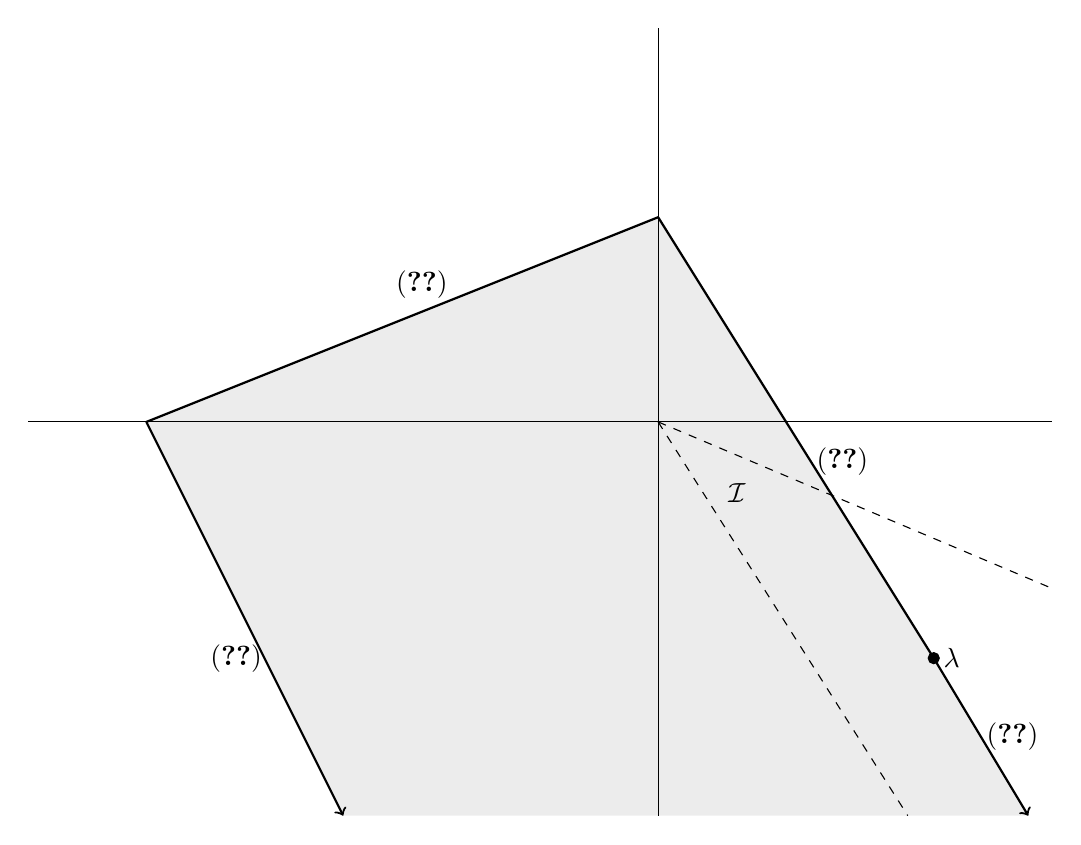
\begin{tikzpicture}
        \filldraw[color=lightgray!30] (47/10,-5) --(3.5,-3) -- (0,26/10) -- (-26/4,0) -- (-16/4,-5);
        \draw[-] (-8,0) -- (5,0);
        \draw[-] (0,-5) -- (0,5);
        %\filldraw[color=lightgray!30] (0,0) -- (5,-2.113) -- (5,-5) -- (3.17,-5) -- (0,0);
        \draw[dashed] (0,0) -- (5,-2.113);
        \draw[dashed] (0,0) -- (3.17,-5);
        \node at (1,-0.9) {$\cI$};
        \draw[fill=black] (3.5,-3) circle (2pt);
        \node[right] at (3.5,-3) {$\lambda$};
        \draw[->,thick] (3.5,-3) -- (47/10,-5);
        \draw[-,thick] (3.5,-3) -- (0,26/10);
        \draw[-,thick] (0,26/10) -- (-26/4,0);
        \draw[->,thick] (-26/4,0) -- (-16/4,-5);
        \node at (4.5,-4) {\eqref{ineq:1}};
        \node at (2.34,-0.5) {\eqref{ineq:2}};
        \node at (-3,1.75) {\eqref{ineq:3}};
        \node at (-5.36,-3) {\eqref{ineq:4}};
      \end{tikzpicture}
    \]
  \end{lemma}
  \begin{proof}
    Following Lemma~\ref{le:imaginary transformations}, we consider even and odd sequences of mutations separately.

    For $k=2j$, $j>0$, and $\lambda\in\cI$, we observe that $\cC_k(\phi_k\lambda)\subset\RR^2$ is given by the inequalities 
    \[ (\dagger)\ x\le u_{2j+1,+}\lambda_1+u_{2j,+}\lambda_2 \qquad\text{and}\qquad (\ddagger)\ -y\le u_{2j,-}\lambda_1+u_{2j-1,-}\lambda_2. \]
    We inductively compute the region $\phi_{2j}^{-1}\cC_{2j}(\phi_{2j}\lambda)$, using Lemma~\ref{le:transformed inequalities} and the equality $\phi_{2j}^{-1}=\phi_2^{-j}$.

    \subsubsection*{Claim:} For $i>0$, $\phi_{2i}^{-1}\cC_{2j}(\phi_{2j}\lambda)$ is the region determined by the inequalities 
    \begin{align*}
      \tag{a} u_{2i,-}x+u_{2i-1,+}y &\le u_{2j,-}\lambda_1+u_{2j-1,+}\lambda_2;\\
      \tag{b} u_{2i+1,-}x+u_{2i,+}y &\le u_{2j+1,-}\lambda_1+u_{2j,+}\lambda_2;\\
      \tag{c} -u_{2i-1,-}x+u_{2i,+}y &\le u_{2j+1,-}\lambda_1+u_{2j,+}\lambda_2;\\
      \tag{d} -u_{2i-1,-}x-u_{2i-2,+}y &\le u_{2j+1,-}\lambda_1+u_{2j,+}\lambda_2.
    \end{align*}

    We see from \eqref{eq:backward two step mutation}, that $\lambda\in\cI$ implies the boundary ray for $\cC_{2j}(\phi_{2j}\lambda)$ corresponding to ($\ddagger$) lies entirely in the region in which $\phi_2^{-1}$ acts according to the matrix $\left[ \begin{array}{cc} -1 & -b\\ c & bc-1 \end{array}\right]$ of determinant 1.
    By Lemma~\ref{le:transformed inequalities}, the inequality ($\ddagger$) transforms into the inequality $cx+y\le u_{2j,-}\lambda_1+u_{2j-1,+}\lambda_2$ which corresponds to (a) with $i=1$.
    Similarly, the boundary ray for $\cC_{2j}(\phi_{2j}\lambda)$ corresponding to ($\dagger$) intersects the three domains of linearity in which $\phi_2^{-1}$ acts according to the matrices $\left[ \begin{array}{cc} -1 & -b\\ c & bc-1 \end{array}\right]$, $\left[ \begin{array}{cc} -1 & -b\\ 0 & -1 \end{array}\right]$, $\left[ \begin{array}{cc} -1 & 0\\ 0 & -1 \end{array}\right]$, each of determinant 1.
    By Lemma~\ref{le:transformed inequalities}, the inequality ($\dagger$) can be seen to transform by these into each of inequalities (b), (c), (d) with $i=1$.
    This establishes the base of an induction on $i$.

    Assuming the inequalities (a)-(d) hold for $k$, we apply Lemma~\ref{le:transformed inequalities} with $\phi_2^{-1}$.
    Both of the boundary rays corresponding to the inequalities (a) and (d) lies entirely in the region where $\phi_2^{-1}$ acts according to the matrix $\left[ \begin{array}{cc} -1 & -b\\ c & bc-1 \end{array}\right]$, also the boundary segment corresponding to (b) intersects this region.
    Thus applying Lemma~\ref{le:transformed inequalities} to (a) gives the inequality 
    \[u_{2i+2,-}x+u_{2i+1,+}y=(u_{3,+}u_{2i,-}-u_{2,-}u_{2i-1,+})x+(u_{2,+}u_{2i,-}-u_{1,-}u_{2i-1,+})y\le u_{2j,-}\lambda_1+u_{2j-1,+}\lambda_2,\]
    which is the inequality (a) for $i+1$ by Lemma~\ref{eq:long Chebyshev recursion}; while applying this to (d) gives the inequality 
    \[-u_{2i+1,-}x-u_{2i,+}y=(-u_{3,+}u_{2i-1,-}+u_{2,-}u_{2i-2,+})x+(-u_{2,+}u_{2i-1,-}+u_{1,-}u_{2i-2,+})y\le u_{2j+1,-}\lambda_1+u_{2j,+}\lambda_2,\]
    which is the inequality (d) for $k+1$ again by Lemma~\ref{eq:long Chebyshev recursion}; finally applying this to (b) gives the inequality 
    \[u_{2i+3,-}x+u_{2i+2,+}y=(u_{3,+}u_{2i+1,-}-u_{2,-}u_{2i,+})x+(u_{2,+}u_{2i+1,-}-u_{1,-}u_{2i,+})y\le u_{2j+1,-}\lambda_1+u_{2j,+}\lambda_2,\]
    which is the inequality (b) for $i+1$.
    Similarly, the boundary segment corresponding to (c) lies entirely in the region where $\phi_2^{-1}$ acts according to the matrix $\left[ \begin{array}{cc} -1 & 0\\ c & -1 \end{array}\right]$.
    Thus applying Lemma~\ref{le:transformed inequalities} to (c) gives the inequality 
    \[-u_{2i+1,-}x-u_{2i,+}y=(u_{1,+}u_{2i-1,-}-u_{2,-}u_{2i,+})x+(-u_{0,+}u_{2i-1,-}-u_{1,-}u_{2i,+})y\le u_{2j+1,-}\lambda_1+u_{2j,+}\lambda_2,\]
    which is the inequality (d) for $i+1$ by Lemma~\ref{eq:long Chebyshev recursion}, in particular we see that the segment determined by (c) and the ray determined by (d) align in the image.
    Lastly, the boundary segment corresponding to (b) also intersects the regions where $\phi_2^{-1}$ acts according to the matrices $\left[ \begin{array}{cc} -1 & -b\\ 0 & -1 \end{array}\right]$ and $\left[ \begin{array}{cc} -1 & 0\\ 0 & -1 \end{array}\right]$ respectively.
    Applying Lemma~\ref{le:transformed inequalities} to (b) with the first matrix gives the inequality 
    \[-u_{2i+1,-}x+u_{2i+2,+}y=(-u_{1,+}u_{2i+1,-}+u_{0,-}u_{2i,+})x+(u_{2,+}u_{2i+1,-}-u_{1,-}u_{2i,+})y\le u_{2j+1,-}\lambda_1+u_{2j,+}\lambda_2,\]
    which is the inequality (c) for $i+1$ by Lemma~\ref{eq:long Chebyshev recursion}, while applying Lemma~\ref{le:transformed inequalities} to (b) with the second matrix gives the inequality 
    \[-u_{2i+1,-}x-u_{2i,+}y\le u_{2j+1,-}\lambda_1+u_{2j,+}\lambda_2,\]
    which again reproduces the inequality (d) and aligns with the previous segment and ray in the image.
    This completes the induction on $i$, proving the Claim and the result for $k$ even.

    For $k=2j+1$, $j>0$, and $\lambda\in\cI$, we get $\cC_{2j+1}(\phi_{2j+1}\lambda)\subset\RR^2$ is given by the inequalities 
    \[ (\dagger')\ -x\le u_{2j+1,+}\lambda_1+u_{2j,+}\lambda_2 \qquad\text{and}\qquad (\ddagger')\ y\le u_{2j+2,-}\lambda_1+u_{2j+1,-}\lambda_2.\]
    Using that $\phi_{2j+1}^{-1}=\phi_2^{-j}\phi_1^{-1}$, we compute the image inductively as above.
    From \eqref{eq:forward mutation 1} and Lemma~\ref{le:imaginary stability}, we see that the boundary ray for $\cC_{2j+1}(\phi_{2j+1}\lambda)$ corresponding to ($\dagger'$) lies entirely in the region in which $\phi_1^{-1}$ acts according to the matrix $\left[ \begin{array}{cc} -1 & 0\\ c & 1 \end{array}\right]$ of determinant $-1$.
    Thus applying Lemma~\ref{le:transformed inequalities}, the inequality ($\dagger'$) is transformed by $\phi_1^{-1}$ into the inequality $x\le u_{2j+1,+}\lambda_1+u_{2j,+}\lambda_2$.
    The boundary ray corresponding to ($\ddagger'$) intersects both domains of linearity for $\phi_1^{-1}$ and thus produces the inequalities
    \[ cx+y\le u_{2j+2,+}\lambda_1+u_{2j+1,+}\lambda_2 \qquad\text{and}\qquad  y\le u_{2j+2,+}\lambda_1+u_{2j+1,+}\lambda_2.\]


    \subsubsection*{Claim:} For $i\ge 0$, $\phi_{2i+1}^{-1}\cC_{2j+1}(\phi_{2j+1}\lambda)$ is the region determined by the inequalities 
    \begin{align*}
      \tag{a$'$} u_{2i+1,-}x+u_{2i,+}y &\le u_{2j+1,-}\lambda_1+u_{2j,+}\lambda_2;\\
      \tag{b$'$} u_{2i+2,-}x+u_{2i+1,+}y &\le u_{2j+2,-}\lambda_1+u_{2j+1,+}\lambda_2;\\
      \tag{c$'$} -u_{2i,-}x+u_{2i+1,+}y &\le u_{2j+2,-}\lambda_1+u_{2j+1,+}\lambda_2;\\
      \tag{d$'$} -u_{2i,-}x-u_{2i-1,+}y &\le u_{2j+2,-}\lambda_1+u_{2j+1,+}\lambda_2.
    \end{align*}
    By essentially the same calculations as above, these inequalities reproduce under the action of $\phi_2^{-1}$ and this completes the proof.
  \end{proof}

  \begin{lemma}
    \label{le:one direction}
    For $\lambda\in\cI\cap\ZZ^2$, 
    \begin{enumerate}
      \item $\cP_+(\lambda):=\bigcap_{i \ge 0}\phi_{t_i}^{-1}\cC_{t_i}(\phi_{t_i}\lambda)$ is the quadrilateral with corner vertices $\lambda$, $(\frac{2-bc-\sqrt{bc(bc-4)}}{2}\lambda_1-\frac{bc+\sqrt{bc(bc-4)}}{2c}\lambda_2,0)$, $(0,\frac{bc+\sqrt{bc(bc-4)}}{2b}\lambda_1+\lambda_2)$, and $(\frac{2-bc-\sqrt{bc(bc-4)}}{2}\lambda_1-b\lambda_2,\lambda_2)$.
      \item $\cP_-(\lambda):=\bigcap_{i \le 0}\phi_{t_i}^{-1}\cC_{t_i}(\phi_{t_i}\lambda)$ is the quadrilateral with corner vertices $\lambda$, $(\lambda_1+\frac{bc+\sqrt{bc(bc-4)}}{2c}\lambda_2,0)$, $(0,-\frac{bc+\sqrt{bc(bc-4)}}{2b}\lambda_1+\frac{2-bc-\sqrt{bc(bc-4)}}{2}\lambda_2)$, and $(\lambda_1,-c\lambda_1+\frac{2-bc-\sqrt{bc(bc-4)}}{2}\lambda_2)$.
    \end{enumerate}
  \end{lemma}
  \begin{proof}
    We prove (1) as (2) is obtained by interchanging $b$ with $c$ and swapping all ordered pairs.  
    We first show that $\cC_{t_0}(\lambda) \cap \phi_{t_i}^{-1}\cC_{t_i}(\phi_{t_i}\lambda)\supsetneq \cC_{t_0}(\lambda) \cap \phi_{t_j}^{-1}\cC_{t_j}(\phi_{t_j}\lambda)$ for $0\le i<j$.
  \end{proof}



\section{Lattice Mutations and Linear Inequalities}


  For $b\in\ZZ$, write $[b]_+=max(b,0)$.
  Given a sign $\varepsilon\in\{\pm1\}$ and $k\in\{1,\ldots,n\}$, define a matrix $E_{k,\varepsilon}=(e_{ij})$ with
  \begin{equation}
    \label{eq:left mutation matrix}
    e_{ij}=\begin{cases} 1 & \text{if $i=j\ne k$;}\\ -1 & \text{if $i=j=k$;}\\ [\varepsilon b_{ik}]_+ & \text{if $i\ne j=k$;}\\ 0 & \text{otherwise;} \end{cases}
  \end{equation}
  and a matrix $F_{k,\varepsilon}=(f_{ij})$ with
  \begin{equation}
    \label{eq:right mutation matrix}
    f_{ij}=\begin{cases} 1 & \text{if $k\ne i=j$;}\\ -1 & \text{if $k=i=j$;}\\ [-\varepsilon b_{kj}]_+ & \text{if $k=i\ne j$;}\\ 0 & \text{otherwise.} \end{cases}
  \end{equation}
  Observe that $E^2_{k,\varepsilon}=\Id$ and $F^2_{k,\varepsilon}=\Id$ for any $k$ and any choice of $\varepsilon$.
  \begin{lemma}
    For $\varepsilon\in\{\pm1\}$ and $k\in\{1,\ldots,n\}$, we have $E_{k,-\varepsilon}E_{k,\varepsilon}=I_n+\varepsilon B^{\bullet k}$ and $E_{k,\varepsilon}-E_{k,-\varepsilon}=\varepsilon B^{\bullet k}$.
  \end{lemma}
  \begin{proof}
    This is immediate from the equality $\varepsilon b_{ij}=[\varepsilon b_{ij}]_+-[-\varepsilon b_{ij}]_+$.
  \end{proof}

  The index $k\in\{1,\ldots,n\}$ also determines a new skew-symmetrizable matrix $\mu_k B=(b'_{ij})$ given by
  \[ b'_{ij}=\begin{cases} -b_{ij} & \text{if $i=k$ or $j=k$;}\\ b_{ij}+[b_{ik}]_+b_{kj}+b_{ik}[-b_{kj}]_+ & \text{otherwise.} \end{cases} \]
  One easily observes that $\mu_k B$ is again skew-symmetrizable using the same matrix $D$.
  \begin{remark}
    Note that $\mu_k B=E_{k,\varepsilon} B F_{k,\varepsilon}$ for $\varepsilon=\pm 1$, the case $\varepsilon=1$ being obvious from the definitions and the case $\varepsilon=-1$ following from the identity $b_{ij}=[b_{ij}]_+-[-b_{ij}]_+$.
  \end{remark}

  To record sequences of these matrix mutations, we introduce the labeled $n$-regular rooted tree $\TT_n$ with root vertex $t_0$ and associate skew-symmetrizable matrices $B^t$ for $t\in\TT_n$ satisfying:
  \begin{itemize}
    \item $B^{t_0}=B$;
    \item if $t,t'\in\TT_n$ are joined by an edge labeled $k$, then $B^{t'}=\mu_k B^t$.
  \end{itemize}

  (DR: I changed to $\RR$ because it didn't seem like we really cared about integer points at the moment, when we try to link up with minors this will need to be added.)
  For $t\in\TT_n$, define $\phi^t_k:\RR^n\to\RR^n$ as the piecewise-linear map
  \[\phi^t_k(\lambda)=\begin{cases} E^t_{k,+}\lambda & \text{if $\lambda_k\ge0$;}\\ E^t_{k,-}\lambda & \text{if $\lambda_k<0$;} \end{cases}\]
  where the entries of $E^t_{k,\varepsilon}$ are given by \eqref{eq:left mutation matrix} with $b^t_{ij}$ in place of $b_{ij}$.
  We leave it as an exercise for the reader to check that $(\phi^t_k)^{-1}=\phi^{t'}_k$ whenever $t,t'\in\TT_n$ are joined by an edge labeled $k$.
  \begin{lemma}
    Suppose $t,t'\in\TT_n$ are joined by an edge labeled $k$.
    If $\mu\in\lambda+\Col(B^t)$, then $\phi^t_k(\mu)\in\phi^t_k(\lambda)+\Col(B^{t'})$.
  \end{lemma}
  \begin{proof}
    Suppose $\mu=\lambda+B^t\alpha$ for some $\alpha\in\RR^n$.
    Let $\varepsilon$ (resp. $\varepsilon'$) be such that $\phi^t_k(\mu)=E^t_{k,\varepsilon}\mu$ (resp. $\phi^t_k(\lambda)=E^t_{k,\varepsilon'}\lambda$).
    Then 
    \[\phi^t_k(\mu)=E^t_{k,\varepsilon}\mu=E^t_{k,\varepsilon}(\lambda+B^t\alpha)=E^t_{k,\varepsilon}\lambda + E^t_{k,\varepsilon} B^t F^t_{k,\varepsilon} F^t_{k,\varepsilon}\alpha=E^t_{k,\varepsilon}\lambda + B^{t'} F^t_{k,\varepsilon}\alpha.\]
    If $\varepsilon'=\varepsilon$, this is equal to $\phi^t_k(\lambda) + B^{t'} F^t_{k,\varepsilon}\alpha$ and so $\phi^t_k(\mu)\in\phi^t_k(\lambda)+\Col(B^{t'})$.
    Otherwise, 
    \[E^t_{k,\varepsilon}\lambda=E^t_{k,\varepsilon'}\lambda+\varepsilon(B^t)^{\bullet k}\lambda=\phi^t_k(\lambda)-\varepsilon(B^{t'})^{\bullet k}\lambda=\phi^t_k(\lambda)-\varepsilon B^{t'} \lambda_k \mathbf{e}_k\]
    and again we see that $\phi^t_k(\mu)\in\phi^t_k(\lambda)+\Col(B^{t'})$.
  \end{proof}





  \section{Rank Two}

  \begin{theorem}
    There are six classes of dominance polytopes.
    \begin{enumerate}
      \item If $\lambda$ lies outside of $\cI$, i.e. if it is the $\bfg$-vector of a cluster monomial, then $\cP(\lambda)$ is the point $\lambda$. 
      \item If $\lambda$ lies in the interior of the cone spanned by the vectors $(2b,-bc-\sqrt{bc(bc-4)})$ and $(2,-c)$, then $\cP(\lambda)$ is the trapezoid with corner vertices $\lambda$, $-\frac{bc+\sqrt{bc(bc-4)}}{2c}\big(\frac{bc+\sqrt{bc(bc-4)}}{2b}\lambda_1+\lambda_2,0\big)$, $\big(0,\frac{bc+\sqrt{bc(bc-4)}}{2b}\lambda_1+\lambda_2\big)$, and $\frac{bc+\sqrt{bc(bc-4)}}{2\sqrt{bc(bc-4)}}\big(-(bc-2)\lambda_1-b\lambda_2,c\lambda_1+2\lambda_2\big)$.
      \item If $\lambda$ lies on the ray spanned by $(2,-c)$, say $\lambda=(2\ell,-c\ell)$, then $\cP(\lambda)$ is the triangle with corner vertices $\lambda$, $\big(2\ell-\frac{bc+\sqrt{bc(bc-4)}}{2}\ell,0\big)$, and $\big(0,\frac{\sqrt{bc(bc-4)}}{b}\ell\big)$.
      \item If $\lambda$ lies in the interior of the cone spanned by the vectors $(2,-c)$ and $(b,-2)$, then $\cP(\lambda)$ is the kite with corner vertices $\lambda$, $\big(\lambda_1+\frac{bc+\sqrt{bc(bc-4)}}{2c}\lambda_2,0\big)$, $\frac{bc+\sqrt{bc(bc-4)}}{2\sqrt{bc(bc-4)}}(2\lambda_1+b\lambda_2,c\lambda_1+2\lambda_2)$, and $\big(0,\frac{bc+\sqrt{bc(bc-4)}}{2b}\lambda_1+\lambda_2\big)$.
      \item If $\lambda$ lies on the ray spanned by $(b,-2)$, say $\lambda=(b\ell,-2\ell)$, then $\cP(\lambda)$ is the triangle with corner vertices $\lambda$, $\big(-\frac{\sqrt{bc(bc-4)}}{c}\ell,0\big)$, and $\big(0,\frac{bc+\sqrt{bc(bc-4)}}{2}\ell-2\ell\big)$.
      \item If $\lambda$ lies in the interior of the cone spanned by the vectors $(b,-2)$ and $(2b,-bc+\sqrt{bc(bc-4)})$, then $\cP(\lambda)$ is the trapezoid with corner vertices $\lambda$, $\big(\lambda_1+\frac{bc+\sqrt{bc(bc-4)}}{2c}\lambda_2,0\big)$, $-\frac{bc+\sqrt{bc(bc-4)}}{2b}\big(0,\lambda_1+\frac{bc+\sqrt{bc(bc-4)}}{2c}\lambda_2\big)$, and $\frac{bc+\sqrt{bc(bc-4)}}{2\sqrt{bc(bc-4)}}\big(2\lambda_1+b\lambda_2,-c\lambda_1-(bc-2)\lambda_2\big)$.
    \end{enumerate}
  \end{theorem}
  \begin{proof}
    Following Lemma~\ref{le:one direction}, we see that the intersection $\cP_+(\lambda)\cap\cP_-(\lambda)$ degenerates to a triangle precisely when
    \[\frac{2-bc-\sqrt{bc(bc-4)}}{2}\lambda_1-\frac{bc+\sqrt{bc(bc-4)}}{2c}\lambda_2=\lambda_1+\frac{bc+\sqrt{bc(bc-4)}}{2c}\lambda_2\]
    or 
    \[\frac{bc+\sqrt{bc(bc-4)}}{2b}\lambda_1+\lambda_2=-\frac{bc+\sqrt{bc(bc-4)}}{2b}\lambda_1+\frac{2-bc-\sqrt{bc(bc-4)}}{2}\lambda_2.\]
    The first equations reduces to $c\lambda_1+2\lambda_2=0$, while the second reduces to $2\lambda_1+b\lambda_2=0$.
    In particular, the rays spanned by $(2,-c)$ and $(b,-2)$ determine this change of state in the dominance regions $\cP(\lambda)$.
  \end{proof}

%  The dominance polygon pointed at $\lambda=(\lambda_1,\lambda_2)$ is the region defined by the following inequalities:
%  \begin{align}
%    -\lambda_1-\frac{b c+\sqrt{b c (b c-4)}}{2 c}\lambda_2+x+\frac{b c+\sqrt{b c (b c-4)}}{2 c}y\geq0
%    \\
%    \frac{b c+\sqrt{b c (b c-4)}}{2 b}\lambda_1+\lambda_2-\frac{b c+\sqrt{b c (b c-4)}}{2 b}x-y\geq0
%    \\
%    -\frac{b c+\sqrt{b c (b c-4)}}{2 b}\lambda_1 - \frac{b c+\sqrt{b c (b c-4)}-2}{2}\lambda_2 + \frac{b c+\sqrt{b c (b c-4)}}{2 b}x-y\geq0
%    \\
%    \frac{b c+\sqrt{b c (b c-4)}-2}{2}\lambda_1+\frac{b c+\sqrt{b c (b c-4)}}{2 c}\lambda_2+x-\frac{b c+\sqrt{b c (b c-4)}}{2 c}y\geq0
%    \\
%    -\frac{b c+\sqrt{b c (b c-4)}}{2 b}\lambda_1-\frac{b c+\sqrt{b c (b c-4)}-2}{2}\lambda_2-\frac{b c-\sqrt{b c (b c-4)}}{2 b}x-y\geq0
%    \\
%    \frac{b c+\sqrt{b c (b c-4)}-2}{2}\lambda_1+\frac{b c+\sqrt{b c (b c-4)}}{2 c}\lambda_2+x+\frac{b c-\sqrt{b c (b c-4)}}{2 c}y\geq0
%  \end{align}
%  Are any of these better forms?
%  \begin{align}
%    (x-\lambda_1)+\frac{b c+\sqrt{b c (b c-4)}}{2 c}(y-\lambda_2)\geq0
%    \\
%    \nonumber \iff \frac{b c-\sqrt{b c (b c-4)}}{2 b}(x-\lambda_1)+(y-\lambda_2)\geq0
%    \\
%    -\frac{b c+\sqrt{b c (b c-4)}}{2 b}(x-\lambda_1)-(y-\lambda_2)\geq0
%    \\
%    \nonumber \iff -(x-\lambda_1)-\frac{b c-\sqrt{b c (b c-4)}}{2 c}(y-\lambda_2)\geq0
%    \\
%    -\frac{b c+\sqrt{b c (b c-4)}}{2}\lambda_2 + \frac{b c+\sqrt{b c (b c-4)}}{2 b}(x-\lambda_1)-(y-\lambda_2)\geq0
%    \\
%    \nonumber \iff -b\lambda_2 + (x-\lambda_1)-\frac{b c-\sqrt{b c (b c-4)}}{2 c}(y-\lambda_2)\geq0
%    \\
%    \frac{b c+\sqrt{b c (b c-4)}}{2}\lambda_1+(x-\lambda_1)-\frac{b c+\sqrt{b c (b c-4)}}{2 c}(y-\lambda_2)\geq0
%    \\
%    \nonumber \iff c\lambda_1+\frac{b c-\sqrt{b c (b c-4)}}{2 b}(x-\lambda_1)-(y-\lambda_2)\geq0
%    \\
%    -c\lambda_1-\frac{b c+\sqrt{b c (b c-4)}}{2}\lambda_2-\frac{b c-\sqrt{b c (b c-4)}}{2 b}(x-\lambda_1)-(y-\lambda_2)\geq0
%    \\
%    \frac{b c+\sqrt{b c (b c-4)}}{2}\lambda_1+b\lambda_2+(x-\lambda_1)+\frac{b c-\sqrt{b c (b c-4)}}{2 c}(y-\lambda_2)\geq0
%  \end{align}
%  Another proposal (I also changed the order of the equations)
%  \begin{align}
%    \frac{b c-\sqrt{b c (b c-4)}}{2 b}(x-\lambda_1)+(y-\lambda_2) & \geq0
%    \\
%    \frac{b c+\sqrt{b c (b c-4)}}{2 b}(x-\lambda_1-b\lambda_2)-(y-\lambda_2) & \geq 0
%    \\
%    -\frac{b c-\sqrt{b c (b c-4)}}{2 b}(x-\lambda_1)-(y-\lambda_2)& \geq c\lambda_1+\frac{b c+\sqrt{b c (b c-4)}}{2b}b\lambda_2
%    \\
%    -(x-\lambda_1)-\frac{b c-\sqrt{b c (b c-4)}}{2 c}(y-\lambda_2)& \geq0
%    \\
%    (x-\lambda_1)-\frac{b c+\sqrt{b c (b c-4)}}{2 c}(y-\lambda_2-c\lambda_1) & \geq 0
%    \\
%    (x-\lambda_1)+\frac{b c-\sqrt{b c (b c-4)}}{2 c}(y-\lambda_2) & \geq -\frac{b c+\sqrt{b c (b c-4)}}{2c}c\lambda_1-b\lambda_2
%  \end{align}
%  Maybe this one:
%  \begin{align}
%    \frac{b c-\sqrt{b c (b c-4)}}{2 b}(x-\lambda_1)+(y-\lambda_2) & \geq0
%    \\
%    \frac{b c+\sqrt{b c (b c-4)}}{2 b}(x-\lambda_1-b\lambda_2)-(y-\lambda_2) & \geq 0
%    \\
%    -\frac{b c-\sqrt{b c (b c-4)}}{2 b}(x-\lambda_1)-(y-\lambda_2)& \geq c\lambda_1+\frac{b c+\sqrt{b c (b c-4)}}{2b}b\lambda_2
%    \\
%    -(x-\lambda_1)-\frac{b c-\sqrt{b c (b c-4)}}{2 c}(y-\lambda_2)& \geq0
%    \\
%    (x-\lambda_1)-\frac{b c+\sqrt{b c (b c-4)}}{2 c}(y-\lambda_2-c\lambda_1) & \geq 0
%    \\
%    (x-\lambda_1)+\frac{b c-\sqrt{b c (b c-4)}}{2 c}(y-\lambda_2) & \geq -\frac{b c+\sqrt{b c (b c-4)}}{2c}c\lambda_1-b\lambda_2
%  \end{align}
%
%  Yet another version:
% 
% {
%    \everymath={\displaystyle}
%  \[
%  \begin{array}{rcccl}
%    -c\lambda_1-\frac{b c+\sqrt{b c (b c-4)}}{2b}b\lambda_2 & \geq & \frac{b c-\sqrt{b c (b c-4)}}{2 b}(x-\lambda_1)+(y-\lambda_2) & \geq & 0
%    \\
%    &  & \frac{b c-\sqrt{b c (b c-4)}}{2 b}(x-\lambda_1)-(y-\lambda_2) & \geq & c\lambda_1
%    \\
%    - b \lambda_2 & \geq & - (x-\lambda_1) + \frac{b c-\sqrt{b c (b c-4)}}{2 c} (y-\lambda_2) 
%    \\
%    0 & \geq & (x-\lambda_1)+\frac{b c-\sqrt{b c (b c-4)}}{2 c}(y-\lambda_2) & \geq &-\frac{b c+\sqrt{b c (b c-4)}}{2c}c\lambda_1-b\lambda_2
%  \end{array}
%\]
%}
%
%Or: (Maybe at this point we can remove $c/c$ and $b/b$)
%
% {
%    \everymath={\displaystyle}
%  \[
%  \begin{array}{rcccl}
%    -c\lambda_1-\frac{b c+\sqrt{b c (b c-4)}}{2b}b\lambda_2 & \geq & \frac{b c-\sqrt{b c (b c-4)}}{2 b}(x-\lambda_1)+(y-\lambda_2) & \geq & 0
%    \\
%    &  & \frac{b c-\sqrt{b c (b c-4)}}{2 b}(x-\lambda_1)-(y-\lambda_2) & \geq & c\lambda_1
%    \\
%    -\frac{b c+\sqrt{b c (b c-4)}}{2c}c\lambda_1-b\lambda_2  & \leq & (x-\lambda_1)+\frac{b c-\sqrt{b c (b c-4)}}{2 c}(y-\lambda_2) & \leq & 0
%    \\
%    & & - (x-\lambda_1) + \frac{b c-\sqrt{b c (b c-4)}}{2 c} (y-\lambda_2)  & \leq & - b \lambda_2
%  \end{array}
%\]
%}
%
%
%Or Or: (Maybe at this point we can remove $c/c$ and $b/b$)
%
%
% The following, and possibly all the one before, has a typo
% {
%    \everymath={\displaystyle}
%    \def\arraystretch{2.8}
%  \[
%  \begin{array}{rcccl}
%    0 & \leq & \frac{b c-\sqrt{b c (b c-4)}}{2 b}(x-\lambda_1)+(y-\lambda_2) & \leq & -c\lambda_1-\frac{b c+\sqrt{b c (b c-4)}}{2b}b\lambda_2
%    \\
%    c\lambda_1 & \leq & \frac{b c-\sqrt{b c (b c-4)}}{2 b}(x-\lambda_1)-(y-\lambda_2)
%    \\
%    0 & \leq &  -(x-\lambda_1)-\frac{b c-\sqrt{b c (b c-4)}}{2 c}(y-\lambda_2) & \leq & \frac{b c+\sqrt{b c (b c-4)}}{2c}c\lambda_1+b\lambda_2
%    \\
%    b \lambda_2 & \leq & (x-\lambda_1) - \frac{b c-\sqrt{b c (b c-4)}}{2 c} (y-\lambda_2)
%  \end{array}
%\]
%}
% {
%    \everymath={\displaystyle}
%    \def\arraystretch{2.8}
%  \[
%  \begin{array}{rcccl}
%    0 & \leq & \frac{b c-\sqrt{b c (b c-4)}}{2 b}(x-\lambda_1)+(y-\lambda_2) & \leq & -c\lambda_1-\frac{b c+\sqrt{b c (b c-4)}}{2b}b\lambda_2
%    \\
%    -c\lambda_1 & \leq & \frac{b c-\sqrt{b c (b c-4)}}{2 b}(x-\lambda_1)-(y-\lambda_2)
%    \\
%    0 & \leq &  -(x-\lambda_1)-\frac{b c-\sqrt{b c (b c-4)}}{2 c}(y-\lambda_2) & \leq & \frac{b c+\sqrt{b c (b c-4)}}{2c}c\lambda_1+b\lambda_2
%    \\
%    b \lambda_2 & \leq & (x-\lambda_1) - \frac{b c-\sqrt{b c (b c-4)}}{2 c} (y-\lambda_2)
%  \end{array}
%\]
%}
  The dominance polygon pointed at $\lambda=(\lambda_1,\lambda_2)$ is the region defined by $x\leq \lambda_1, y\geq\lambda_2$, and the following inequalities:
 {
    \everymath={\displaystyle}
    \def\arraystretch{2.8}
  \[
  \begin{array}{rcccl}
    0 & \leq & \frac{b c-\sqrt{b c (b c-4)}}{2 b}(x-\lambda_1)+(y-\lambda_2) & \leq & \max\left(-c\lambda_1-\frac{b c+\sqrt{b c (b c-4)}}{2b}b\lambda_2,0\right)
    \\
    \min\left(-c\lambda_1,0\right) & \leq & \frac{b c-\sqrt{b c (b c-4)}}{2 b}(x-\lambda_1)-(y-\lambda_2) & \leq & 0
    \\
    0 & \leq &  -(x-\lambda_1)-\frac{b c-\sqrt{b c (b c-4)}}{2 c}(y-\lambda_2) & \leq & \max\left(\frac{b c+\sqrt{b c (b c-4)}}{2c}c\lambda_1+b\lambda_2,0\right)
    \\
    \min\left(b \lambda_2,0\right) & \leq & (x-\lambda_1) - \frac{b c-\sqrt{b c (b c-4)}}{2 c} (y-\lambda_2) & \leq & 0
  \end{array}
\]
}

\section{The Total Domination Polyhedron}

  Define the \emph{total domination polyhedron} $\cD:=\{(\lambda,\mu):\mu\in\cP(\lambda)\}$, i.e. this is the set of all pairs where $\lambda$ dominates $\mu$.
  Write $\pi_1:\cD\to\RR^n$ for the projection to $\lambda$ and $\pi_2:\cD\to\RR^n$ for the projection to $\mu$.
  \begin{itemize}
    \item Is it a polyhedron?
    \item The lemma below might suggest so.  
      Indeed, if it is, by the Decomposition Theorem, we can write $\cD$ as the Minkowski sum of a polyhedral cone (almost certainly $\cI$) and a convex polytope (what is it?).
      I am ignoring that it should really be the union of this polyhedron with a plane if the previous sentence holds any water.
    \item Actually, we might need to take the union of several polyhedra to account for the variations in the fibers $\pi_1^{-1}(\lambda)$.
  \end{itemize}

  Is the following result true beyond rank 2?
  \begin{lemma}
    For $\mu\in\RR^2$, $\pi_2^{-1}(\mu)$ is a translate of the imaginary cone $\cI$ or the union of such with a single point.
  \end{lemma}
  \begin{proof}
    For $\mu$ in the second quadrant, the vertex of this cone should be given by $\lambda=(\lambda_1,\lambda_2)$ where
    \[\lambda_1=\frac{2b\mu_2-4\mu_1}{bc-4+\sqrt{bc(bc-4)}} \qquad \text{and} \qquad \lambda_2=\frac{2c\mu_1-4\mu_2}{bc-4+\sqrt{bc(bc-4)}}.\]
    (This comes from setting $\mu$ to be the vertex opposite $\lambda$ inside the dominance region $\cP(\lambda)$ and then solving for $\lambda$.)
  \end{proof}
  \begin{remark}
    We want to understand what the curve is that results when we have $\mu$ lie along the unit circle, this should be possible by plugging $(\cos(\theta),\sin(\theta))$ into this formula for $\lambda$ and seeing what ellipse we get.
  \end{remark}


\section{Proof of Theorem~\ref{th:dominance vertices}}


\section{Proof of Theorem~\ref{th:maximum support}}

  \begin{theorem}\label{th:Newton polygons}\cite[Proposition~4.1]{LLZ}, \cite[Corollary~3.5]{LLZ2}
    For $(a_1,a_2)\in\ZZ^2$, the smallest (possibly degenerate) lattice quadrilateral $R_{a_1,a_2}$ containing the support of $x[a_1,a_2]$ is determined as follows.
    \begin{enumerate}
      \item If $a_1 \leq 0$ and $a_2 \leq 0$, then $R_{a_1,a_2} = \{(-a_1,-a_2)\}$.
      \item If $a_1 \leq 0 < a_2$, then $R_{a_1,a_2} = \{(p_1,-a_2): -a_1\leq p_1\leq -a_1+ba_2\}$.
      \item If $a_2 \leq 0 < a_1$, then $R_{a_1,a_2} = \{(-a_1,p_2): -a_2 \leq p_2 \leq -a_2+ca_1\}$.
      \item If $0<ba_2\leq a_1$, then $R_{a_1,a_2}=\left\{(p_1,p_2): -a_1\le p_1\le -a_1+ba_2,\; -a_2\le p_2\le -a_2-cp_1\right\}$.
      \item If $0<ca_1\leq a_2$, then $R_{a_1,a_2}=\left\{(p_1,p_2): -a_1\le p_1\le -a_1-bp_2,\; -a_2\le p_2\le -a_2+ca_1\right\}$.
      \item If $0 < a_1 < ba_2$ and $0 < a_2 < ca_1$, then
      $$\aligned
      R_{a_1,a_2}=&\bigg\{(p_1,p_2)\bigg|\; -a_1\le p_1<0,\; -a_2\le p_2<\Big(\frac{a_2}{a_1}-c\Big)p_1\bigg\}\\
      &\bigcup\bigg\{(p_1,p_2): -a_1\le p_1<\Big(\frac{a_1}{a_2}-b\Big)p_2,\; -a_2\le p_2<0\bigg\}\\
      &\hspace{1.35em}\bigcup\Big\{(-a_1+ba_2,-a_2),(-a_1,-a_2+ca_1)\Big\}.
      \endaligned
      $$
    \end{enumerate}
    Moreover, if $z\in\cA(b,c)$ is pointed at $(a_1,a_2)$ with support contained in $R_{a_1,a_2}$, then $z=x[a_1,a_2]$. 
  \end{theorem}

\section{The affine case}
  \label{sec:affine}
  In this section we compare our main result with the construction of \cite{RSW19} in the case $b=c=2$.
  We show that the continuous family of bases constructed there is precisely the deformation family constructed by \cite{Qin}.


  We want to show that our continuous family of generalized minors from \cite[Theorem 4.6]{RSW19} coincide with the family of bases constructed in \cite[Theorem 1.2.1]{Qin19}.
  
  This boils down to show, for any $n>1$, that
  \begin{enumerate}
    \item 
      the set of $\bfg$-vectors that are dominated by $n\omega^\circ$ with respect to any seed is 
      \[
        \left\{(n-2r)\omega^\circ \right\}_{r\in\left[1,\left\lfloor\frac{1}{2}\right\rfloor\right]}
      \]
  
    \item
      we can choose a specific basis and rewrite the last formula in \cite[Proposition 4.4]{RSW19} as in \cite[Theorem 1.2.1]{Qin19} with coefficients being functions of the point $\bfa\in(\kk^\times)^n$. 
  \end{enumerate}
  
  For a partition $\lambda \vdash n$ let $e_\lambda$, $s_\lambda$, and $m_\lambda$ denote the elementary, Shur, and monomial symmetric functions associated to the partition $\lambda$ evaluated at $\bfa$.
  Recall that $m_{1^{(n)}} = s_{1^{(n)}} = e_n$.
  
  \begin{lemma}
    For every $r\in\left[1,\left\lfloor\frac{1}{2}\right\rfloor\right]$ we have $m_{1^{(n)}} S_{\bfa,r} = m_{2^{(r)},1^{(n-2r)}}$.
  \end{lemma}
  \begin{proof}
    This is immediate from the definition.
  \end{proof}
  
  Let $F_{n\omega^\circ}^\Delta$, $F_{n\omega^\circ}^{gr}$, $F_{n\omega^\circ}^{tr}$, and $F_{n\omega^\circ}^{ge}$ be the $F$-polynomials of the generalized minor, greedy basis element, triangular basis element, and generic basis element with $\bfg$-vector $n\omega^\circ$.
  We think of $F$-polynomials as polynomials in the variables $u_1$ and $u_2$.
  
  I did not try yet to prove (1) but it should be straightforward.
  It suffices to establish (2) for the $F$-polynomials.
  
  \begin{proposition}
    \[
      m_{1^{(n)}} F_{n\omega^\circ}^\Delta
      =
      \sum_{r=0}^{\lfloor \frac{n}{2} \rfloor}
      m_{2^{(k)},1^{(n-2r)}}
      u_1^r u_2^r
      F_{(n-2r)\omega^\circ}^{ge}
    \]
  \end{proposition}
  \begin{proof}
    From \cite[Proposition 4.4]{RSW19} we get the following expression for $F_{n\omega^\circ}^\Delta$:
    \[
       F_{n\omega^\circ}^\Delta 
       =
       \sum_{0 \le k \le \ell \le n}
       \sum_{r=0}^\ell
       {\ell -r \choose k}
       {n-2r \choose \ell-r}
       S_{\bfa,r}
       u_1^\ell u_2^{\ell-k}.
    \]
    From the second binomial coefficient we deduce that $n-2r$ is positive so the second sum runs up to $\lfloor \frac{n}{2} \rfloor$.
    We compute
    \begin{align*}
      m_{1^{(n)}}  F_{n\omega^\circ}^\Delta 
      &
      =
      \sum_{0 \le k \le \ell \le n}
      \sum_{r=0}^{\lfloor \frac{n}{2} \rfloor}
      {\ell -r \choose k}
      {n-2r \choose \ell-r}
      m_{2^{(r)},1^{(n-2r)}}
      u_1^\ell u_2^{\ell-k}
      \\
      &=
      \sum_{r=0}^{\lfloor \frac{n}{2} \rfloor}
      m_{2^{(r)},1^{(n-2r)}}
      u_1^r u_2^r
      \sum_{0 \le k \le \ell \le n}
      {\ell -r \choose k}
      {n-2r \choose \ell-r}
      u_1^{\ell-r} u_2^{\ell-r-k}
      \\
      &=
      \sum_{r=0}^{\lfloor \frac{n}{2} \rfloor}
      m_{2^{(r)},1^{(n-2r)}}
      u_1^r u_2^r
      F_{(n-2r)\omega^\circ}^{ge}.
    \end{align*}
    The last identity follows immediately by comparing with the formula for generic basis elements in \cite{RSW19}.
    \saySS{Thank you Dylan for fixing my stupidity.}
  \end{proof}
  
  We do not need the following two formulas but I think they are still neat.
  \begin{conjecture}
    \begin{align*} 
      m_{1^{(n)}} F_{n\omega^\circ}^\Delta
      &=
      \sum_{r=0}^{\lfloor \frac{n}{2} \rfloor}
      s_{2^{(k)},1^{(n-2r)}}
      u_1^r u_2^r
      F_{(n-2r)\omega^\circ}^{tr}
      \\&=
      \sum_{r=0}^{\lfloor \frac{n}{2} \rfloor}
      e_{r,n-r}
      u_1^r u_2^r
      F_{(n-2r)\omega^\circ}^{gr}
    \end{align*}
  \end{conjecture}

  \begin{thebibliography}{XXX}

    \bibitem{lee-li-zelevinsky}
      K.~Lee, L.~Li, A.~Zelevinsky: Greedy elements in rank 2 cluster algebras. Selecta Math. \textbf{20} (2014), pp.~57--82.

    \bibitem{rupel}
      D.~Rupel: Rank two non-commutative Laurent phenomenon and pseudo-positivity.  Algebraic Combinatorics, \textbf{2} (2019) no. 6, pp.~1239--1273. \href{https://doi.org/10.5802/alco.81}{DOI: 10.5802/alco.81}.
  \end{thebibliography}


  
\end{document}

  \section{Bases From Compatible Pairs on Dyck Paths}
  \sayDR{This is a bit of a repetition of the above introduction to Dyck paths, but with slightly different goals it seemed that a modified exposition was more appropriate.}
  For $a_1,a_2\in\ZZ_{\ge0}$, choose a Dyck path $D$ in the lattice rectangle $[0,a_1]\times[0,a_2]$.
  When we wish to emphasize the upper right bounding corner we will write $D[a_1,a_2]$.
  Consider $D$ as the totally ordered set of its edges along the natural labeling from $(0,0)$ to $(a_1,a_2)$.
  It may be convenient to identify $D$ with the ordered set $[1,a_1+a_2]$.
  Write $D=D_1\sqcup D_2$, where $D_1=\{h_1,\ldots,h_{a_1}\}$ is the set of horizontal edges and $D_2=\{v_1,\ldots,v_{a_2}\}$ is the set of vertical edges.
  Define the \emph{height}, $\hgt(h)$ for $h\in D_1$, as one more than the number of $v\in D_2$ with $v<h$.
  Define the \emph{depth}, $\dpt(v)$ for $v\in D_2$, as the number of $h\in D_1$ with $h<v$.
  \begin{remark}
    The seemingly different conventions for computing height and depth provide uniformity later.
    Indeed, the vertical edges immediately following $h_d$ have depth $d$, while this convention allows the horizontal edges immediately preceding $v_\ell$ to similarly be said to have height $\ell$.
  \end{remark}

  Observe that the data of $D$ is just the data of a bipartition of a finite totally ordered set $D=D_1\sqcup D_2$.
  Given a Dyck path $D=D_1\sqcup D_2$ in the lattice rectangle $[0,a_1]\times[0,a_2]$, write $\bar{D}=\bar{D}_1 \sqcup \bar{D}_2$ for the Dyck path (under the identification with $[1,a_1+a_2]$) in the lattice rectangle $[0,a_2]\times[0,a_1]$ with $\bar{D}_1=a_1+a_2+1-D_2$ and $\bar{D}_2=a_1+a_2+1-D_1$.
  This operation can be visualized as transposing the Dyck path.

  Given any quantity or object $P$ whose definition depends on $b$ and $c$, write $\vv{P}$ for the same quantity or object defined with $b$ and $c$ interchanged.
  In particular, we have $\vv{u}_{m,\varepsilon}=u_{m,-\varepsilon}$ for any $m$ and any $\varepsilon=\pm1$.

  \subsection{Structure of Dyck Paths}

  Write $D^{max}=D^{max}[a_1,a_2]$ for the maximal Dyck path in the lattice rectangle $[0,a_1]\times[0,a_2]$, i.e. $D^{max}$ never crosses above the diagonal line joining $(0,0)$ to $(a_1,a_2)$ and any lattice point above $D^{max}$ also lies above the diagonal.
  Observe that $\bar{D}^{max}[a_1,a_2]=D^{max}[a_2,a_1]$.

  \begin{definition}
    Call a Dyck path $D$ 
    \begin{itemize}
      \item \emph{horizontally-adapted to $b$} if no vertical edge of $D$ is immediately preceded by more than $b$ horizontal edges;
      \item \emph{vertically-adapted to $c$} if no horizontal edge of $D$ is immediately followed by more than $c$ vertical edges.
    \end{itemize}
  \end{definition}

  \begin{definition}
    \label{def:Dyck path mutations}
    Given a Dyck path $D=D[a_1,a_2]$ which is vertically-adapted to $c$, define a Dyck path $\mu_{1,c}(D)$ inside the lattice rectangle $[0,ca_1-a_2]\times[0,a_1]$ by replacing each horizontal edge of $D$, together with the $r$ vertical edges which immediately follow it, by $c-r$ horizontal edges followed by a vertical edge.
    This provides a canonical identification of the horizontal edges of $D$ with the vertical edges of $\mu_{1,c}(D)$, this identification is again denoted by $\mu_{1,c}$.

    Given a Dyck path $D=D[a_1,a_2]$ which is horizontally-adapted to $b$, define a Dyck path $\mu_{2,b}(D)$ inside the lattice rectangle $[0,a_2]\times[0,ba_2-a_1]$ by replacing each vertical edge of $D$, together with the $r$ horizontal edges which immediately precede it, by a horizontal edge followed by $b-r$ vertical edges.
    This provides a canonical identification of the vertical edges of $D$ with the horizontal edges of $\mu_{2,b}(D)$, this identification is again denoted by $\mu_{2,b}$.
  \end{definition}
  \begin{remark}
    Observe that $\mu_{1,a}$ and $\mu_{2,a}$ are inverse for any $a\ge1$ whenever they are defined.
  \end{remark}

  The following result is proven in \cite[Lemma 2.4]{rupel} with appropriate notation changes, c.f. Theorem~\ref{th:dominant Dyck path recursion} for a slight modification and explicit proof.
  \begin{lemma}\mbox{}
    \label{le:maximal Dyck path recursion}
    \begin{enumerate}
      \item If $a_2 < c a_1$, then $\mu_{1,c}\big(D^{max}[a_1,a_2]\big)=D^{max}[ca_1-a_2,a_1]$.
      \item If $a_1 < b a_2$, then $\mu_{2,b}\big(D^{max}[a_1,a_2]\big)=D^{max}[a_2,ba_2-a_1]$.
    \end{enumerate}
  \end{lemma}

  As an immediate consequence, we determine the structure of certain maximal Dyck paths.
  We introduce the following notation for convenience:
  \[d_m:=\begin{cases} b & \text{if $m$ is even;}\\ c & \text{if $m$ is odd;}\end{cases} \qquad \text{and} \qquad \vv{d}_m:=\begin{cases} c & \text{if $m$ is even;}\\ b & \text{if $m$ is odd;}\end{cases}\]
  The following was proven in \cite[Corollary 2.6]{rupel} and follows by a simple induction using Lemma~\ref{le:maximal Dyck path recursion}.
  \begin{corollary}
    Assume $b,c\ge2$ (this can be dropped with extra notation and slight modification).
    Then, for $\varepsilon=\pm1$ and $m\ge1$, the maximal Dyck path $D^{m,\varepsilon}:=D^{max}[u_{m,\varepsilon},u_{m-1,-\varepsilon}]$ can be constructed as follows:
    \begin{itemize}
      \item $D^{1,\varepsilon}$ consists of a single horizontal edge;
      \item $D^{2,\varepsilon}$ consists of $d_2$ horizontal edges followed by a vertical edge;
      \item for $m\ge3$, $D_{m,\varepsilon}$ consists of $d_m - 1$ copies of $D^{m-1,\varepsilon}$ followed by a copy of $D^{m-1,\varepsilon}$ with its first $D^{m-2,\varepsilon}$ removed;
    \end{itemize}
    and the maximal Dyck path $\vv{\bar{D}}^{m,\varepsilon}:=D^{max}[u_{m-1,\varepsilon},u_{m,-\varepsilon}]$ can be constructed as follows:
    \begin{itemize}
      \item $\vv{\bar{D}}^{1,\varepsilon}$ consists of a single vertical edge;
      \item $\vv{\bar{D}}^{2,\varepsilon}$ consists of a horizontal edge followed by $\vv{d}_2$ vertical edges;
      \item for $m\ge3$, $\vv{\bar{D}}^{m,\varepsilon}$ consists of a copy of $\vv{\bar{D}}^{m-1,\varepsilon}$ with its last $\vv{\bar{D}}^{m-2,\varepsilon}$ removed followed by $\vv{d}_m - 1$ copies of $\vv{\bar{D}}^{m-1,\varepsilon}$.
    \end{itemize}
  \end{corollary}

  Our main interest will be with the following Dyck paths.
  \begin{definition}
    \label{def:dominant Dyck path}
    For $a_1,a_2\in\ZZ_{\ge0}$ with $(-a_1+ba_2,-a_2)\in\cI$, define the \emph{dominant Dyck path} $D^{dom}=D^{dom}[a_1,a_2]$ to be the maximal Dyck path starting from $(0,0)$ and terminating at $(a_1,a_2)$ while staying below the lines $y=\frac{bc+\sqrt{bc(bc-4)}}{2b}x$ and $y-a_2=\frac{bc-\sqrt{bc(bc-4)}}{2b}(x-a_1)$.

    For $a_1,a_2\in\ZZ_{\ge0}$ with $(-a_2,-a_1+ca_2)\in\cI'$, define the \emph{dual dominant Dyck path} $\vv{D}^{dom}=\vv{D}^{dom}[a_1,a_2]$ to be the maximal Dyck path starting from $(0,0)$ and terminating at $(a_1,a_2)$ while staying below the lines $y=\frac{bc+\sqrt{bc(bc-4)}}{2c}x$ and $y-a_2=\frac{bc-\sqrt{bc(bc-4)}}{2c}(x-a_1)$.
  \end{definition}
  \begin{remark}
    \label{rem:intersection}
    The lines defining $D^{dom}[a_1,a_2]$ meet at the point 
    \[m_{a_1,a_2}:=\left( \frac{2ba_2-\big(bc-\sqrt{bc(bc-4)}\big)a_1}{2\sqrt{bc(bc-4)}} , \frac{\big(bc+\sqrt{bc(bc-4)}\big)a_2-2ca_1}{2\sqrt{bc(bc-4)}} \right).\]
  \end{remark}

  To understand the structure of the dominant Dyck paths, it will be convenient to consider their initial and final segments separately.
  \begin{definition}
    For $s>0$, define the \emph{Dyck path prefix} $\overrightarrow{D}^s$ as the maximal Dyck path with $s$ vertical edges starting from $(0,0)$ and terminating at $(d,s)$ while staying below the line $y=\frac{bc+\sqrt{bc(bc-4)}}{2b}x$, where $d=d_s=\left\lceil s \frac{bc-\sqrt{bc(bc-4)}}{2c}\right\rceil$.
    Call this $d$ the \emph{depth} of $s$.

    For $t>0$, define the \emph{Dyck path suffix} $\overleftarrow{D}^t$ as the maximal Dyck path with $t$ horizontal edges starting from $(0,0)$ and terminating at $(t,h)$ while staying below the line $y-h=\frac{bc-\sqrt{bc(bc-4)}}{2b}(x-t)$, where $h=h_t=\left\lceil t \frac{bc-\sqrt{bc(bc-4)}}{2b}\right\rceil$.
    Call this $h$ the \emph{height} of $t$.
  \end{definition}
  \begin{remark}
    There often exist multiple choices of $s$ with a given depth $d$ and multiple choices of $t$ with a given height $h$.
  \end{remark}
  \sayDR{ToDo: describe the analogue of Corollary 7.5 for the Dyck path prefixes and suffixes.}

  The following result will be useful for showing that the Dyck path prefixes and suffixes behave properly.
  \begin{lemma}
    For $s>0$, the Dyck path prefix $\overrightarrow{D}^s$ ends in a vertical edge.
    Similarly, for $t>0$, the Dyck path suffix $\overleftarrow{D}^t$ begins with a horizontal edge.
  \end{lemma}

  \begin{lemma}
    For $s,t>0$, $\overrightarrow{D}^s=D^{dom}[d_s,s]$ and $\overleftarrow{D}^t=D^{dom}[t,h_t]$.
  \end{lemma}
  \begin{proof}
    Is this obvious?
    %Following Remark~\ref{rem:intersection}, the intersection point of the lines defining $D^{dom}[d_s,s]$ is given by
    %\[m_{d_s,s}=\left( \frac{2bs-\big(bc-\sqrt{bc(bc-4)}\big)d_s}{2\sqrt{bc(bc-4)}} , \frac{\big(bc+\sqrt{bc(bc-4)}\big)s-2cd_s}{2\sqrt{bc(bc-4)}} \right).\]
    %By definition of $d_s$, we have
    %\[\frac{\big(bc+\sqrt{bc(bc-4)}\big)s-2cd_s}{2\sqrt{bc(bc-4)}} \le \frac{\big(bc+\sqrt{bc(bc-4)}\big)s-\big(bc-\sqrt{bc(bc-4)}\big)s}{2\sqrt{bc(bc-4)}} = s\]
  \end{proof}

  \begin{lemma}
    For any $s,t>0$, the Dyck path prefix $\overrightarrow{D}^s$ and Dyck path suffix $\overleftarrow{D}^t$ are both horizontally-adapted to $b$ and vertically-adapted to $c$.
  \end{lemma}
  \begin{proof}
    Observe that $\frac{c}{2}<\frac{bc+\sqrt{bc(bc-4)}}{2b}<c$.
    This shows that $\overrightarrow{D}^s$ cannot contain more than $c$ consecutive vertical edges following a horizontal edge and so $\overrightarrow{D}^s$ must be vertically-adapted to $c$.
    In addition, we see that $\overrightarrow{D}^s$ can only contain consecutive horizontal edges if $c=1$, in which case there are at most two consecutive horizontal edges preceding any vertical edge.
    But, since we assume $bc\ge4$, that would imply $b\ge4$ and so $\overrightarrow{D}^s$ must be horizontally-adapted to $b$.
  \end{proof}

  \begin{theorem}
    \label{th:dominant Dyck path recursion}
    For $a_1,a_2\in\ZZ_{\ge0}$ with $(-a_1+ba_2,-a_2)\in\cI$, we have $\mu_{1,c}\big(D^{dom}[a_1,a_2]\big)=\vv{D}^{dom}[ca_1-a_2,a_1]$ and $\mu_{2,b}\big(D^{dom}[a_1,a_2]\big)=\vv{D}^{dom}[a_2,ba_2-a_1]$.
  \end{theorem}
  \begin{proof}
    We prove the result for $\mu_{1,c}$ as the result for $\mu_{2,b}$ immediately follows from $\mu_{1,b}$ being its inverse.
    Write $D'$ for the Dyck path $\mu_{1,c}\big(D^{dom}[a_1,a_2]\big)$ and observe that by construction $D'$ has $ca_1-a_2$ horizontal edges and $a_1$ vertical edges.
    Write $v'_1,\ldots,v'_{a_1}$ for the vertical edges of $D'$ with $v'_k$ immediately preceded by $r_k$ horizontal edges.
    We have to show (i) that every lattice point on $D'$ stays below the lines 
    \[y=\frac{bc+\sqrt{bc(bc-4)}}{2c}x \qquad \text{and} \qquad y-a_1=\frac{bc-\sqrt{bc(bc-4)}}{2c}\big(x-(ca_1-a_2)\big)\]
    while (ii) any lattice point above $D'$ is also above one of these lines.

    If there exists $t$ so that $v'_t$ passes above the line $y=\frac{bc+\sqrt{bc(bc-4)}}{2c}x$, then
    \[ \frac{t}{\sum\limits_{k=1}^t r_k} > \frac{bc+\sqrt{bc(bc-4)}}{2c} \]
    or, rearranging, we have
    \[ \frac{\sum\limits_{k=1}^t r_k}{t} < \frac{2c}{bc+\sqrt{bc(bc-4)}} = \frac{bc-\sqrt{bc(bc-4)}}{2b} \]
    or
    \[ \frac{bc+\sqrt{bc(bc-4)}}{2b} < \frac{ct-\sum\limits_{k=1}^t r_k}{t} = \frac{\sum\limits_{k=1}^t (c-r_k)}{t}. \]
    But this states that the subpath of $D^{dom}[a_1,a_2]$ consisting of the first $t$ horizontal edges and all their trailing vertical edges passes above the line $y=\frac{bc+\sqrt{bc(bc-4)}}{2b}x$, contrary to the definition.

    If there exists $t$ so that $v'_t$ passes above the line $y-a_1=\frac{bc-\sqrt{bc(bc-4)}}{2c}\big(x-(ca_1-a_2)\big)$, then
    \[ \frac{bc-\sqrt{bc(bc-4)}}{2c} > \frac{a_1-t}{ca_1-a_2-\sum\limits_{k=1}^t r_k} \]
    or, rearranging, we have
    \[ \frac{ca_1-a_2-\sum\limits_{k=1}^t r_k}{a_1-t} > \frac{2c}{bc-\sqrt{bc(bc-4)}} = \frac{bc+\sqrt{bc(bc-4)}}{2b} \]
    or
    \[ \frac{bc-\sqrt{bc(bc-4)}}{2b} > \frac{ c(a_1-t) - \big(ca_1-a_2-\sum\limits_{k=1}^t r_k\big)}{a_1-t} = \frac{a_2-\sum\limits_{k=1}^t (c-r_k)}{a_1-t}. \]
    But this states that the subpath of $D^{dom}[a_1,a_2]$ consisting of the first $t$ horizontal edges and all their trailing vertical edges passes above the line $y-a_2=\frac{bc-\sqrt{bc(bc-4)}}{2b}(x-a_1)$, contrary to the definition.

    This proves (i), analogous calculations establish (ii). 
  \end{proof}

  Apart from being the prefix and suffix for the dominant Dyck path, the Dyck paths $\overrightarrow{D}^s$ and $\overleftarrow{D}^t$ can be observed inside the maximal Dyck paths defining cluster variables as follows.
  \begin{lemma}\mbox{}
    \begin{itemize}
      \item For $s>0$ and any $m \ge 2$ so that $s < u_{m,-}$, the Dyck path prefix $\overrightarrow{D}^s$ is an initial segment of the maximal Dyck path $D^{max}[u_{m-1,+},u_{m,-}]$.
      \item For $t>0$ and any $m \ge 2$ so that $t < u_{m,+}$, the Dyck path suffix $\overleftarrow{D}^t$ is a final segment of the maximal Dyck path $D^{max}[u_{m,+},u_{m-1,-}]$.
    \end{itemize}
  \end{lemma}

  \begin{lemma}\mbox{}
    \begin{enumerate}
      \item Choose a width $t>0$ and $a_1 \ge t$.
        Then there exists a unique $s$ of depth $a_1-t$ so that $\overrightarrow{D}^s \sqcup \overleftarrow{D}^t$ is the dominant Dyck path $D^{dom}[a_1,a_2]$ with $a_2=s+\left\lceil t \frac{bc-\sqrt{bc(bc-4)}}{2b}\right\rceil$.
      \item Choose a height $s>0$ and $a_2 \ge s$.
        Then there exists a unique $t$ of height $a_2-s$ so that $\overrightarrow{D}^s \sqcup \overleftarrow{D}^t$ is the dominant Dyck path $D^{dom}[a_1,a_2]$ with $a_1=\left\lceil s \frac{bc-\sqrt{bc(bc-4)}}{2c}\right\rceil+t$.
    \end{enumerate}
  \end{lemma}
  \begin{remark}
    The decomposition of $D^{dom}[a_1,a_2]$ as $\overrightarrow{D}^s \sqcup \overleftarrow{D}^t$ is not uniquely determined by $a_1$ and $a_2$.
    However, there exists at most two choices of $s$ and $t$ for which such a decomposition holds.
  \end{remark}

  \begin{lemma}
    \label{le:floors and ceilings}
    For any real number $x$ and any real number $r>1$, we have
    \[\lfloor x\rfloor \le \left\lfloor \lceil xr \rceil \frac{1}{r} \right\rfloor \le \lceil x\rceil \qquad \text{and} \qquad \lfloor x\rfloor \le \left\lceil \lfloor xr \rfloor \frac{1}{r} \right\rceil \le \lceil x\rceil.\]
  \end{lemma}
  \begin{proof}
    Observe that
    \[xr\le \lceil xr \rceil < xr+1 \qquad \text{and} \qquad xr-1 < \lfloor xr \rfloor \le xr\]
    and so
    \[x\le \lceil xr \rceil \frac{1}{r} < x+\frac{1}{r} \qquad \text{and} \qquad x-\frac{1}{r} < \lfloor xr \rfloor \frac{1}{r} \le x.\]
    Since $0<\frac{1}{r}<1$, the result follows.
  \end{proof}

  The following result describes the possible decomposition of the dominant Dyck path into its prefix and suffix subpaths.
  The intersection point from Remark~\ref{rem:intersection} is a useful point of reference.
  \begin{proposition}
    \label{prop:dominant Dyck path decomposition}
    For $a_1,a_2\in\ZZ_{\ge0}$ with $(-a_1+ba_2,-a_2)\in\cI$, the dominant Dyck path $D^{dom}[a_1,a_2]$ is the concatenation of $\overrightarrow{D}^s$ followed by $\overleftarrow{D}^t$ for any choice of $s$ and $t$ satisfying $a_2-s=\left\lceil t \frac{bc-\sqrt{bc(bc-4)}}{2b}\right\rceil$ and $a_1-t=\left\lceil s \frac{bc-\sqrt{bc(bc-4)}}{2c}\right\rceil$.
    In this case, the pair of $s$ and $t$ will be one of the following:
    \begin{align}
      \label{eq:lower bounds}
      s=\left\lfloor\frac{\big(bc+\sqrt{bc(bc-4)}\big)a_2 - 2 c a_1}{2\sqrt{bc(bc-4)}}\right\rfloor\qquad &\text{and}\qquad t=\left\lfloor\frac{\big(bc+\sqrt{bc(bc-4)}\big)a_1 - 2 b a_2}{2\sqrt{bc(bc-4)}}\right\rfloor\\
      s=\left\lfloor\frac{\big(bc+\sqrt{bc(bc-4)}\big)a_2 - 2 c a_1}{2\sqrt{bc(bc-4)}}\right\rfloor\qquad &\text{and}\qquad t=\left\lceil\frac{\big(bc+\sqrt{bc(bc-4)}\big)a_1 - 2 b a_2}{2\sqrt{bc(bc-4)}}\right\rceil\\
      \label{eq:upper bounds}
      s=\left\lceil\frac{\big(bc+\sqrt{bc(bc-4)}\big)a_2 - 2 c a_1}{2\sqrt{bc(bc-4)}}\right\rceil\qquad &\text{and}\qquad t=\left\lceil\frac{\big(bc+\sqrt{bc(bc-4)}\big)a_1 - 2 b a_2}{2\sqrt{bc(bc-4)}}\right\rceil
    \end{align}
    If two such decompositions exist, they will be of the form \eqref{eq:lower bounds} and \eqref{eq:upper bounds}.
  \end{proposition}
  \begin{remark}
    The irrationality of the slopes defining the Dyck path prefixes and suffixes makes it difficult to predict for a given choice of $a_1$ and $a_2$ precisely which of these choice of $s$ and $t$ will produce the desired equalities.
  \end{remark}
  \begin{proof}
    (In progress)

    For $s=\left\lfloor\frac{\big(bc+\sqrt{bc(bc-4)}\big)a_2 - 2 c a_1}{2\sqrt{bc(bc-4)}}\right\rfloor$, by Lemma~\ref{le:floors and ceilings} we have
    \[\left\lfloor \frac{2 b a_2 -\big(bc-\sqrt{bc(bc-4)}\big) a_1}{2\sqrt{bc(bc-4)}} \right\rfloor \le \left\lceil s \frac{bc-\sqrt{bc(bc-4)}}{2c} \right\rceil \le \left\lceil \frac{2 b a_2 -\big(bc-\sqrt{bc(bc-4)}\big) a_1}{2\sqrt{bc(bc-4)}} \right\rceil\]
    since $0<\frac{bc-\sqrt{bc(bc-4)}}{2c}<1$.
    It follows that
    \[ a_1 - \left\lceil \frac{2 b a_2 -\big(bc-\sqrt{bc(bc-4)}\big) a_1}{2\sqrt{bc(bc-4)}} \right\rceil \le a_1 - \left\lceil s \frac{bc-\sqrt{bc(bc-4)}}{2c} \right\rceil \le a_1 - \left\lfloor \frac{2 b a_2 -\big(bc-\sqrt{bc(bc-4)}\big) a_1}{2\sqrt{bc(bc-4)}} \right\rfloor\]
    and so
    \[ \left\lfloor \frac{ \big(bc+\sqrt{bc(bc-4)}\big) a_1 - 2 b a_2 }{2\sqrt{bc(bc-4)}} \right\rfloor \le a_1 - \left\lceil s \frac{bc-\sqrt{bc(bc-4)}}{2c} \right\rceil \le \left\lceil \frac{ \big(bc+\sqrt{bc(bc-4)}\big) a_1 - 2 b a_2 }{2\sqrt{bc(bc-4)}} \right\rceil\]
    with one of these inequalities being an equality.

    If the left hand inequality is an equality, we take $t=\left\lfloor\frac{\big(bc+\sqrt{bc(bc-4)}\big)a_1 - 2 b a_2}{2\sqrt{bc(bc-4)}}\right\rfloor$.

    The desired equalities can be rewritten in the form 
    \[s=a_2-\left\lceil t \frac{bc-\sqrt{bc(bc-4)}}{2b}\right\rceil=\left\lfloor a_2 - t \frac{bc-\sqrt{bc(bc-4)}}{2b}\right\rfloor\]
    and
    \[t=a_1-\left\lceil s \frac{bc-\sqrt{bc(bc-4)}}{2c}\right\rceil=\left\lfloor a_1 - s \frac{bc-\sqrt{bc(bc-4)}}{2c}\right\rfloor.\]
    Combining these, we seek $s$ and $t$ satisfying
    \[s=\left\lfloor a_2 - \left\lfloor a_1 - s \frac{bc-\sqrt{bc(bc-4)}}{2c}\right\rfloor \frac{bc-\sqrt{bc(bc-4)}}{2b}\right\rfloor\]
    and
    \[t=\left\lfloor a_1 - \left\lfloor a_2 - t \frac{bc-\sqrt{bc(bc-4)}}{2b}\right\rfloor \frac{bc-\sqrt{bc(bc-4)}}{2c}\right\rfloor.\]
  \end{proof}

  \subsection{Compatibility}
  The results of this section can mostly be found in \cite{lee-li-zelevinsky,rupel}.
  However since we work in arbitrary Dyck paths instead of just the maximal ones, some results and proofs will need to be adapted.

  For $e \le e'\in D$, write $ee'$ for the subpath of $D$ beginning with $e$ and ending with $e'$.
  When $e=e'$, we take $ee'$ to be the subpath consisting of only the edge $e$.
  \begin{definition}
    For $H\sqcup V\subset D$ with $H\subset D_1$ and $V\subset D_2$ together with a subpath $ee'\subset D$, define the \emph{horizontal shadow statistic}:
    \begin{equation}
      \label{eq:horizontal shadow statistic}
      f_H(ee')=-|ee' \cap D_2|+c|ee'\cap H|
    \end{equation}
    and the \emph{vertical shadow statistic}:
    \begin{equation}
      \label{eq:vertical shadow statistic}
      f_V(ee')=-|ee' \cap D_1|+b|ee'\cap V|.
    \end{equation}
  \end{definition}
  \begin{remark}
    Observe that the shadow statistics are additive with respect to concatenation of subpaths.
  \end{remark}

  A key notion from \cite{lee-li-zelevinsky} is that of ``compatible subsets of a maximal Dyck path'', this construction immediately generalizes to arbitrary Dyck paths as follows.
  \begin{definition}
    Consider $H\sqcup V\subset D$ with $H\subset D_1$ and $V\subset D_2$.
    For $h\in H$ and $v\in V$ with $h<v$, call the path $hv$ \emph{compatible} if there exists an edge $e\in hv$ such that one of the following conditions is satisfied:
    \begin{equation}
      \label{eq:HGC}
      \tag{HGC} e\ne v \quad \text{and} \quad f_H(he)=0;
    \end{equation}
    \begin{equation}
      \label{eq:VGC}
      \tag{VGC} e\ne h \quad \text{and} \quad f_V(ev)=0.
    \end{equation}
    Call the subset $H\sqcup V$ \emph{compatible} if every path $hv$ with $h\in H$ and $v\in V$ is compatible.
    Write $\cC_D$ for the collection of all compatible subsets of $D$.
    Given a subset $H\subset D_1$, write $\cC_D(H)$ for the collection of all $V\subset D_2$ for which $H\sqcup V\in\cC_D$.
    Define $\cC_D(V)$ for $V\subset D_2$ similarly.
  \end{definition}
  \begin{remark}
    In the construction of the greedy basis, it is necessary to consider $D$ as a closed cycle by identifying $(0,0)$ with $(a_1,a_2)$ and allowing subpaths $ee'$ with $e'<e$ to ``wrap around'' $D$ in the obvious way.
    When we wish to emphasize that this condition should be imposed, we denote the Dyck path $D$ instead by $D_\WA$.
    Following \cite[Remark 2.21]{rupel}, for $D^{m,\varepsilon}$ and $\vv{\bar{D}}^{m,\varepsilon}$ the wrap around condition does not restrict compatibility and can thus safely be omitted.
  \end{remark}

  The crucial result from \cite{lee-li-zelevinsky} can be stated as follows: if a Dyck path $D$ is vertically-adapted to $c$ (resp. horizontally adapted to $b$), then there is a bijection between certain compatible subsets of $D$ and certain compatible subsets of $\mu_{1,c}(D)$ (resp. of $\mu_{2,b}(D)$).
  The main step in the proof that needs to be adapted to the general situation is the following.
  For $e \le h\in D$ with $h=h_d\in D_1$, write $eh^{\!\uparrow}$ for the subpath $eh$ together with all vertical edges of depth $d$ immediately following $h$.
  For $v \le e\in D$ with $v=v_\ell\in D_2$, write ${}^\leftarrow\!\!\! ve$ for the subpath $ve$ together with all horizontal edges of height $\ell$ immediately preceding $v$.
  \begin{lemma}\mbox{}
    \label{le:shadow statistic recursion}
    \begin{enumerate}
      \item Suppose the Dyck path $D$ is vertically-adapted to $c$ and let $D'=\mu_{1,c}(D)$ with $D'_2=\{v'_1,\ldots,v'_{a_1}\}$.
        For $H\subset D_1$, define $V'\subset D'_2$ by $V'=D'_2\setminus \mu_{1,c}(H)$.
        Then for any $h_i \le h_j \in D_1$, we have $f_H(h_i h_j^{\!\uparrow})=-\vv{f}_{V'}({}^\leftarrow\!\!\! v'_i v'_j)$.
      \item Suppose the Dyck path $D$ is horizontally-adapted to $b$ and let $D''=\mu_{2,b}(D)$ with $D''_1=\{h''_1,\ldots,h''_{a_2}\}$.
        For $V\subset D_2$, define $H''\subset D''_1$ by $H''=D''_1\setminus \mu_{2,b}(V)$.
        Then for any $v_i \le v_j \in D_2$, we have $f_V({}^\leftarrow\!\!\! v_i v_j)=-\vv{f}_{H''}(h''_i {h''_j}^{\!\uparrow})$.
    \end{enumerate}
  \end{lemma}
  \begin{proof}
    Claim (2) is immediate from claim (1). 
    By definition, we have 
    \begin{align*}
      -\vv{f}_{V'}({}^\leftarrow\!\!\! v'_iv'_j)&=|{}^\leftarrow\!\!\! v'_i v'_j \cap D'_1|-c|{}^\leftarrow\!\!\! v'_i v'_j \cap V'|\\
      &=|{}^\leftarrow\!\!\! v'_i v'_j \cap D'_1|-c\big|{}^\leftarrow\!\!\! v'_i v'_j \cap \big(D'_2\setminus \mu_{1,c}(H)\big)\big|\\
      &=|{}^\leftarrow\!\!\! v'_i v'_j \cap D'_1|-c|{}^\leftarrow\!\!\! v'_i v'_j \cap D'_2|+c\big|{}^\leftarrow\!\!\! v'_i v'_j \cap \mu_{1,c}(H)\big|.
    \end{align*}
    But, by construction of $\mu_{1,c}(D)$ and since $\mu_{2,c}(D')=D$, we have
    \[\big|{}^\leftarrow\!\!\! v'_i v'_j \cap \mu_{1,c}(H)\big|=|h_i h_j^{\!\uparrow} \cap H| \qquad \text{and} \qquad c|{}^\leftarrow\!\!\! v'_i v'_j \cap D'_2|-|{}^\leftarrow\!\!\! v'_i v'_j \cap D'_1|=|h_i h_j^{\!\uparrow} \cap D_2|\]
    giving
    \[-\vv{f}_{V'}({}^\leftarrow\!\!\! v'_iv'_j)=-|h_i h_j^{\!\uparrow} \cap D_2|+c|h_i h_j^{\!\uparrow} \cap H|=f_H(h_i h_j^{\!\uparrow})\]
    as desired.
  \end{proof}

  The desired bijection of compatible subsets is constructed in terms of certain subpaths determined from each compatible subset.
  \begin{definition}
    \label{def:shadows}
    For $H\sqcup V\subset D$ with $H\subset D_1$ and $V\subset D_2$, define the \emph{shadow paths} as follows:
    \begin{itemize}
      \item For $h\in D_1$, write $D(h;H)$ for the shortest subpath $he \subset D$ with $f_H(he)=0$ or, if no such subpath exists, set $D(h;H)=hv_{a_2}$.
      \item For $v\in D_2$, write $D(v;V)$ for the shortest subpath $ev \subset D$ with $f_V(ev)=0$ or, if no such subpath exists, set $D(v;V)=h_1 v$.
    \end{itemize}
    Write 
    \[D(H):=\bigcup_{h\in H} D(h;H) \qquad \text{and} \qquad D(V):=\bigcup_{v\in V} D(v;V).\]
    Define the \emph{shadow} of $H$ (resp. the \emph{shadow} of $V$) as the set $\sh_D(H):=D(H)\cap D_2$ (resp.~$\sh_D(V):=D(V)\cap D_1$) and the \emph{local shadow} of $h\in H$ (resp. of $v\in V$) as the set $\sh_D(h;H)=D(h;H)\cap D_2$ (resp. $\sh_D(v;V)=D(v;V)\cap D_1$).
  \end{definition}

  The proofs of the following results are identical to the proof of the analogous results from \cite{lee-li-zelevinsky,rupel} for maximal Dyck paths.
  \begin{lemma}
    \label{le:shadow statistics}
    Consider $H\sqcup V\subset D$ with $H\subset D_1$ and $V\subset D_2$.
    \begin{enumerate}
      \item For $h\in H$, take $he$ to be the path $D(h;H)$.
        The following hold:
        \begin{enumerate}
          \item for any proper subpath $he'\subsetneq he$, we have $f_H(he')>0$;
          \item if $f_H(he)=0$, then for any proper subpath $e'e\subsetneq he$, we have $f_H(e'e)<0$;
          \item $e\in V$.
        \end{enumerate}
      \item For $v\in V$, take $ev$ to be the path $D(v;V)$.
        The following hold:
        \begin{enumerate}
          \item for any proper subpath $e'v\subsetneq ev$, we have $f_V(e'v)>0$;
          \item if $f_V(ev)=0$, then for any proper subpath $ee'\subsetneq ev$, we have $f_V(ee')<0$;
          \item $e\in H$.
        \end{enumerate}
    \end{enumerate}
  \end{lemma}
  \begin{remark}
    Observe that the subset $V$ has no influence on the claim of (1) and the subset $H$ has no influence on the claim of (2).
  \end{remark}

  \begin{definition}
    Given two Dyck paths $D,D'$ in the lattice rectangle $[0,a_1]\times[0,a_2]$, write $D'\succ D$ if no lattice point of $D'$ lies below a lattice point of $D$.
  \end{definition}
  \begin{remark}
    Equivalently, $D'\succ D$ if no lattice point of $D'$ lies to the right of a lattice point of $D$.
  \end{remark}

  \begin{proposition}
    Let $D,D'$ be two Dyck paths in the lattice rectangle $[0,a_1]\times[0,a_2]$ with $D'\succ D$.
    Identify $D_1$ with $D'_1$ and $D_2$ with $D'_2$ along the natural left-to-right ordering.
    For subsets $H\subset D_1$ and $V\subset D_2$, write $H'\subset D'_1$ and $V'\subset D'_2$ for the corresponding subsets under the identification above.
    If $(H,V) \in \cC_D$, then $(H',V') \in \cC_{D'}$.
  \end{proposition}
  \begin{proof}
    It suffices, by induction, to show that the result holds if $D'$ is an immediate successor of $D$, i.e. when a single pair of a horizontal followed by a vertical is replaced by a vertical followed by a horizontal.
    Assume $D'$ is obtained from $D$ in this way, say with horizontal edge $h_i$ and vertical edge $v_j$ satisfying $v_j=h_i+1$ in $D$ replaced by the vertical edge $v'_j$ and the horizontal edge $h'_i$ satisfying $h'_i=v'_j+1$ in $D'$.

    Consider $(H,V) \in \cC_D$.
    For $h\in H$ and $v\in V$, write $h'\in H'$ and $v'\in V'$ for the corresponding edges.
    We claim that the condition \eqref{eq:HGC} (resp. \eqref{eq:VGC}) being satisfied for the path $hv$ in $D$ implies the same condition is satisfied for the path $h'v'$ in $D'$.

    Suppose \eqref{eq:HGC} is satisfied for the path $hv$ and write $D(h;H)=he$ for $e\in V$ with $e<v$.
    If $h_i,v_j\notin D(h;H)$, then under the identification with $D'$ we have $D(h';H')=D(h;H)$ and \eqref{eq:HGC} is satisfied for the path $h'v'$.
    Alternatively, since $e\in V$, we must have both $h_i,v_j\in D(h;H)$.
    If $h_i\notin H$, then again we have $D(h';H')=D(h;H)$ and \eqref{eq:HGC} is satisfied for the path $h'v'$.
    Thus, we assume $h_i\in H$.

    We begin by assuming $h_i\ne h$.
    This gives two possibilities for $D(h';H')$ depending on $D(h'_i;H')$.
    First, observe that $D(h_i;H)$ is a proper subpath of $h_ie$, for otherwise $f_H(h_ie)=0$ and, by the additivity of $f_H$, $he$ would not be the shortest subpath with $f_H(he)=0$.
    Thus, if $D(h_i;H)$ is followed by at least two vertical edges inside $D(h;H)$, we again have $D(h';H')=D(h;H)$ and \eqref{eq:HGC} is satisfied for the path $h'v'$.
    Otherwise, $D(h';H')$ is an initial subpath of $D(h;H)$ under the identification of $D'$ with $D$ and again \eqref{eq:HGC} is satisfied for the path $h'v'$.

    Now if $h_i=h$...
  \end{proof}

  \begin{corollary}
    Consider $H\sqcup V\subset D$ with $H\subset D_1$ and $V\subset D_2$.
    \begin{enumerate}
      \item For $h\in H$ and a vertical edge $v\in D(h;H)$, the condition \eqref{eq:HGC} is not satisfied for the path $hv$ but for any $V\in\cC_D(H)$ the condition \eqref{eq:VGC} is satisfied for the path $hv$.
        In particular, $D(v;V)$ is a proper subpath of $hv$ for any $V\in\cC_D(H)$.
      \item For $v\in V$ and a horizontal edge $h\in D(v;V)$, the condition \eqref{eq:VGC} is not satisfied for the pair $hv$ but for any $H\in\cC_D(V)$ the condition \eqref{eq:HGC} is satisfied for the path $hv$.
        In particular, $D(h;H)$ is a proper subpath of $hv$ for any $H\in\cC_D(V)$.
    \end{enumerate}
  \end{corollary}

  \begin{lemma}\mbox{}
    \begin{enumerate}
      \item For $H\subset D_1$ and $h,h'\in H$, the local shadows $\sh_D(h;H)$ and $\sh_D(h';H)$ are either disjoint or one is contained in the other.
      \item For $V\subset D_2$ and $v,v'\in V$, the local shadows $\sh_D(v;V)$ and $\sh_D(v';V)$ are either disjoint or one is contained in the other.
    \end{enumerate}
  \end{lemma}

  \begin{definition}
    Consider $H\sqcup V\subset D$ with $H\subset D_1$ and $V\subset D_2$.
    \begin{enumerate}
      \item Define $\rsh_D(H)\subset\sh_D(H)$, the \emph{remote shadow} of $H$, by removing for each $d\in[1,a_1]$ the first (up to) $c$ vertical edges of depth $d$ immediately following $h_d$.
      \item Define $\rsh_D(H)\subset\sh_D(H)$, the \emph{remote shadow} of $V$, by removing for each $\ell\in[0,a_2-1]$ the first (up to) $b$ horizontal edges of height $\ell$ immediately preceding $v_{\ell+1}$.
    \end{enumerate}
  \end{definition}

  \begin{lemma}\mbox{}
    \begin{enumerate}
      \item For $H\subset D_1$, $V\in\cC_D(H)$ if and only if $V$ is disjoint from $\sh_D(H)\setminus\rsh_D(H)$ and one of the conditions \eqref{eq:HGC} or \eqref{eq:VGC} is satisfied for each path $hv$ with $h\in H$ and $v\in\rsh_D(H)$.
      \item For $V\subset D_2$, $H\in\cC_D(V)$ if and only if $H$ is disjoint from $\sh_D(V)\setminus\rsh_D(V)$ and one of the conditions \eqref{eq:HGC} or \eqref{eq:VGC} is satisfied for each path $hv$ with $h\in\rsh_D(V)$ and $v\in V$.
    \end{enumerate}
  \end{lemma}

  \begin{definition}
    For $H\subset D_1$, write $\cC_D^{rsh}(H)$ for the subset of $V\in\cC_D(H)$ with $V\subset\rsh_D(H)$.
    For $V\subset D_2$, write $\cC_D^{rsh}(V)$ for the subset of $H\in\cC_D(V)$ with $H\subset\rsh_D(V)$.
  \end{definition}

  \begin{definition}
    Consider $H\sqcup V\subset D$ with $H\subset D_1$ and $V\subset D_2$.
    \begin{enumerate}
      \item For $1 \le j < d \le a_1$ with $h_j\in H$, denote by $\rsh_D(H)_{j;d}$ the set of all $v\in\rsh_D(H)$ of depth $d$ such that $v\in\sh(h_j;H)$ and $h_j$ is the first horizontal edge before $v$ with this property.
        Define the \emph{local remote shadow} of the edge $h_j$ by $\rsh_D(h_j;H):=\bigsqcup\limits_{d\in[j+1,a_1]} \rsh_D(H)_{j;d}$.
      \item For $1 \le \ell <  k \le a_2$ with $v_k\in V$, denote by $\rsh_D(V)_{k;\ell}$ the set of all $h\in\rsh_D(V)$ of height $\ell$ such that $h\in\sh(v_k;V)$ and $v_k$ is the first vertical edge after $h$ with this property.
        Define the \emph{local remote shadow} of the edge $v_k$ by $\rsh_D(v_k;V):=\bigsqcup\limits_{\ell\in[1,k-1]} \rsh_D(V)_{k;\ell}$.
    \end{enumerate}
  \end{definition}

  As shown in \cite{lee-li-zelevinsky} for maximal Dyck paths, the remote shadow can be characterized as follows.
  \begin{lemma}
    Consider $H\sqcup V\subset D$ with $H\subset D_1$ and $V\subset D_2$.
    \begin{enumerate}
      \item For $1 \le d < j \le a_1$, we have $\rsh_D(H)_{j;d} \ne \varnothing$ if and only if $f_H(h'h_d^{\!\uparrow}) < 0 < f_H(h_jh^{\!\uparrow})$ for every pair of consecutive horizontal edges $h<h'$ in the path $h_j h_d^{\!\uparrow}$.
      \item For $1 \le \ell < k \le a_2$, we have $\rsh_D(V)_{k;\ell} \ne \varnothing$ if and only if $f_V({}^\leftarrow\!\!\! v_\ell v) < 0 < f_V({}^\leftarrow\!\!\! v' v_k)$ for every pair of consecutive vertical edges $v<v'$ in the path ${}^\leftarrow\!\!\! v_\ell v_k$.
    \end{enumerate}
  \end{lemma}

  \begin{lemma}
    Consider $H\sqcup V\subset D$ with $H\subset D_1$ and $V\subset D_2$.
    \begin{enumerate}
      \item Let $1 \le d < j \le a_1$ and suppose $\rsh_D(H)_{j;d} \ne \varnothing$, then
        \[|\rsh_D(H)_{j;d}| = \min\limits_{h_j \le h < h' \le h_d} \min\big( -f_H(h'h_d^{\!\uparrow}) , f_H(h_jh^{\!\uparrow}) \big).\]
      \item Let $1 \le \ell < k \le a_2$ and suppose $\rsh_D(V)_{k;\ell} \ne \varnothing$, then
        \[|\rsh_D(V)_{k;\ell}| = \min\limits_{v_\ell \le v < v' \le v_k} \min\big( -f_V({}^\leftarrow\!\!\! v_\ell v) , f_V({}^\leftarrow\!\!\! v' v_k) \big).\]
    \end{enumerate}
  \end{lemma}
  
  Then the following result immediately follows from Lemma~\ref{le:shadow statistic recursion}.
  \begin{corollary}\mbox{}
    \label{cor:remote shadows}
    \begin{enumerate}
      \item Suppose the Dyck path $D$ is vertically-adapted to $c$ and let $D'=\mu_{1,c}(D)$ with $D'_2=\{v'_1,\ldots,v'_{a_1}\}$.
        For $H\subset D_1$, define $V'\subset D'_2$ by $V'=D'_2\setminus \mu_{1,c}(H)$.
        Then, for $1 \le d < j \le a_1$, we have $|\rsh_D(H)_{j;d}|=|\rsh_{D'}(V')_{d;j}|$.
      \item Suppose the Dyck path $D$ is horizontally-adapted to $b$ and let $D''=\mu_{2,b}(D)$ with $D''_1=\{h''_1,\ldots,h''_{a_2}\}$.
        For $V\subset D_2$, define $H''\subset D''_1$ by $H''=D''_1\setminus \mu_{2,b}(V)$.
        Then, for $1 \le \ell < k \le a_2$, we have $|\rsh_D(V)_{k;\ell}|=|\rsh_{D''}(H'')_{\ell;k}$.
    \end{enumerate}
  \end{corollary}

  In the results below, we keep the notation and assumptions from Corollary~\ref{cor:remote shadows}.
  It follows that, for $H\subset D_1$ and $1 \le d < j \le a_1$, we may define an order-reversing bijection $\theta^H_{j;d} : \rsh_D(H)_{j;d} \to \rsh_{D'}(V')_{d;j}$.
  Similarly, for $V\subset D_2$ and $1 \le \ell < k \le a_2$, we may define an order-reversing bijection $\theta^V_{k;\ell} : \rsh_D(V)_{k;\ell} \to \rsh_{D''}(H'')_{\ell;k}$.
  \begin{definition}\mbox{}
    \begin{enumerate}
      \item For $H\subset D_1$ and $V \subset \rsh_D(H)$, define $\Omega_H(V) \subset \rsh_{D'}(V')$ by
        \[\Omega_H(V)=\{\theta^H_{j;d}(v) : v \in \rsh_D(H)_{j;d}, 1 \le d < j \le a_1\}.\]
      \item For $V\subset D_2$ and $H \subset \rsh_D(V)$, define $\Omega_V(H) \subset \rsh_{D''}(H'')$ by
        \[\Omega_V(H)=\{\theta^V_{k;\ell}(h) : h \in \rsh_D(V)_{k;\ell}, 1 \le \ell < k \le a_2\}.\]
    \end{enumerate}
  \end{definition}

  \begin{lemma}\mbox{}
    \begin{enumerate}
      \item Consider $H\subset D_1$ and $V \subset \rsh_D(H)$.
        Suppose $h'=\theta^H_{j;d}(v)$ for $v\in V$.
        Then $f_{\Omega_H(V)}(h'v'_d)=f_V(h_j v)$.
      \item Consider $V\subset D_2$ and $H \subset \rsh_D(V)$.
        Suppose $v''=\theta^V_{k;\ell}(h)$ for $h\in H$.
        Then $f_{\Omega_V(H)}(h''_\ell v'')=f_V(h v_k)$.
    \end{enumerate}
  \end{lemma}

  The following equivalence of compatibilities is the main result we need.
  \begin{corollary}\mbox{}
    \begin{enumerate}
      \item For $H \subset D_1$ and $V \subset \rsh_D(H)$, we have $V\in\cC_D(H)$ if and only if $\Omega_H(V)\in\cC_{D'}(V')$.
      \item For $V \subset D_2$ and $H \subset \rsh_D(V)$, we have $H\in\cC_D(V)$ if and only if $\Omega_V(H)\in\cC_{D''}(H'')$.
    \end{enumerate}
  \end{corollary}

  We associate to $D$ the element $x_D\in\ZZ_{\ge0}[x_1^{\pm1},x_2^{\pm1}]$ defined as follows
  \[x_D:=x_1^{-a_1} x_2^{-a_2} \sum_{H\sqcup V\in\cC_D} x_1^{b|V|} x_2^{c|H|}.\]

  \begin{theorem}[\cite{lee-li-zelevinsky}]
    For $(a_1,a_2)=(u_{m,+},u_{m-1,-})$ or $(u_{m-1,+},u_{m,-})$ for $m\ge1$, the element $x_{D^{max}[a_1,a_2]}$ is a non-initial cluster variable.
    Otherwise, the element $x_{D^{max}_\WA[a_1,a_2]}$ is an element of the greedy basis
  \end{theorem}

  \begin{lemma}
    Suppose there are two factorizations
    \[x_D=x_1^{-a_1} x_2^{-a_2} \sum_{t=0}^{a_2}\sum_{k=0}^{a_1} \nu_{k,t} x_1^{bt}(1+x_2^c)^{a_1-k}=x_1^{-a_1} x_2^{-a_2} \sum_{s=0}^{a_1}\sum_{\ell=0}^{a_2} \theta_{s,\ell} x_2^{cs}(1+x_1^b)^{a_2-\ell},\]
    where $\nu_{k,t}$ is the number of subsets $V\subseteq_t D_2$ with $|\sh_D(V)|=k$ and $\theta_{s,\ell}$ is the number of subsets $H\subseteq_s D_1$ with $|\sh_D(H)|=\ell$.
    Then 
    \[\sum_{k=0}^{a_1-s} {a_1-k\choose s} \nu_{k,t}=\sum_{\ell=0}^{a_2-t} {a_2-\ell\choose t} \theta_{s,\ell}\]
    for all possible $s$ and $t$.
  \end{lemma}
  \begin{question}
    How do such expressions behave under mutations?
  \end{question}

  \begin{lemma}
    Choose $a_1,a_2\in\ZZ_{\ge0}$.
    For $D^{st}:=D_1\sqcup D_2$ with $D_2=[1,a_2]$ and $D_1=[1,a_1]+a_2$, the element $x_{D^{st}}$ coincides with the corresponding standard monomial basis element.
  \end{lemma}

  \begin{definition}
    Suppose $D^{dom}[a_1,a_2]$ decomposes as $\overrightarrow{D}^s \sqcup \overleftarrow{D}^t$.
    Call a pair of subsets $H \sqcup V$ \emph{piecewise compatible} if the intersections with $\overrightarrow{D}^s$ and $\overleftarrow{D}^t$ are compatible on the subpaths.
  \end{definition}

  \begin{theorem}
    Suppose $H \sqcup V$ is a piecewise compatible subset of $D^{dom}[a_1,a_2]$.
    \begin{itemize}
      \item If the last vertical edge of $\overrightarrow{D}^s$ is contained in $V$, then $H \sqcup V$ is compatible.
      \item If the first horizontal edge of $\overleftarrow{D}^t$ is contained in $H$, then $H \sqcup V$ is compatible.
    \end{itemize}
  \end{theorem}

\end{document}
